%% !TeX program = xelatex
%% 부득이하게 pdflatex을 사용해야 할 경우 위의 magic comment를 제거하십시오.

%%%%%%%%%%%%%%%%%%%%%%%%%%%%%%%%%%%%%%%%%%%%%%%%%%%%%%%%%%%%%%%%%%%%%%%%%%%%%%%%%
%%%  LaTeX document class of the thesis of the Gyeonggi Science High School   %%%
%%%  Last edition 2015.11.13 by Chinook Mok                                   %%%
%%%  Continously being modified by gshslatexintro after 2016.02.02.           %%%
%%%  Check the latest version at : latex.gs.hs.kr                             %%%
%%%  Also refer to https://www.facebook.com/gshstexsociety                    %%%
%%%%%%%%%%%%%%%%%%%%%%%%%%%%%%%%%%%%%%%%%%%%%%%%%%%%%%%%%%%%%%%%%%%%%%%%%%%%%%%%%

\documentclass{gshs_thesis}
\graphicspath{{images/}}
% 이곳에 필요한 별도의 패키지들을 적어넣으시오.
%\usepackage{...}
\usepackage{verbatim} % for commment, verbatim environment
\usepackage{spverbatim} % automatic linebreak verbatim environment
%\usepacakge{indentfirst}
\usepackage{tikz}
%\tikzset{
%	image label/.style={
%		every node/.style={
			%fill=black,
			%text=white,
%			font=\sffamily\scriptsize,
%			anchor=south west,
%			xshift=0,
%			yshift=0,
%			at={(0,0)}
%		}
%	}
%}
\usepackage{amsmath}
\usepackage{amsfonts}
\usepackage{amssymb}
\usepackage{float}
\usepackage{graphicx}
\usepackage{tabularx}
\usepackage{multirow}
\usepackage{booktabs}
\usepackage{longtable}
\usepackage{gensymb}
%\usepackage{subcaption}
%\usepackage{floatrow}
%\usepackage{pict2e}

\usepackage{pgfplots}
\pgfplotsset{
	compat=newest,
	label style={font=\sffamily\scriptsize},
	ticklabel style={font=\sffamily\scriptsize},
	legend style={font=\sffamily\tiny},
	major tick length=0.1cm,
	minor tick length=0.05cm,
	every x tick/.style={black},
}

\usetikzlibrary{shapes}
\usetikzlibrary{plotmarks}
\usepackage{listings}
\usepackage{hologo}
\usepackage{makecell}


\lstset{
	basicstyle=\small\ttfamily,
	columns=flexible,
	breaklines=true
}

\citation
\bibdata



% -----------------------------------------------------------------------
%                   이 부분은 수정하지 마시오.
% -----------------------------------------------------------------------
\titleheader{졸업논문청구논문}
\school{과학영재학교 경기과학고등학교}
\approval{위 논문은 과학영재학교 경기과학고등학교 졸업논문으로\\
졸업논문심사위원회에서 심사 통과하였음.}
\chairperson{심사위원장}
\examiner{심사위원}
\apprvsign{(인)}
\korabstract{초 록}
\koracknowledgement{감사의 글}
\korresearches{연 구 활 동}

%: ----------------------------------------------------------------------
%:                  논문 제목과 저자 이름을 입력하시오
% ----------------------------------------------------------------------
\title{단결정 페로브스카이트의 위치에 따른 PL측정을 통한 waveguiding effect의 원인분석} %한글 제목
\engtitle{Analysis of waveguiding effect by PL measurement according to the position of single crystal perovskite} %영문 제목
\korname{김 주 원} %저자 이름을 한글로 입력하시오 (글자 사이 띄어쓰기)
\engname{Kim, Ju Won} %저자 이름을 영어로 입력하시오 (family name, personal name)
\chnname{金 宙 源} %저자 이름을 한자로 입력하시오 (글자 사이 띄어쓰기)
\studid{17024} %학번을 입력하시오

%------------------------------------------------------------------------
%                  심사위원과 논문 승인 날짜를 입력하시오
%------------------------------------------------------------------------
\advisor{Park, Kie Hyun}  %지도교사 영문 이름 (family name, personal name)
\judgeone{정 문 석} %심사위원장
\judgetwo{김 제 흥}   %심사위원1
\judgethree{박 기 현} %심사위원2(지도교사)
\degreeyear{2019}   %졸업 년도
\degreedate{2019}{7}{21} %논문 승인 날짜 양식

%------------------------------------------------------------------------
%                  논문제출 전 체크리스트를 확인하시오
%------------------------------------------------------------------------
\checklisttitle{[논문제출 전 체크리스트]} %수정하지 마시오
\checklistI{1. 이 논문은 내가 직접 연구하고 작성한 것이다.} %수정하지 마시오
% 이 항목이 사실이라면 다음 줄 앞에 "%"기호 삽입, 다다음 줄 앞의 "%"기호 제거하시오
%\checklistmarkI{$\square$}
\checklistmarkI{$\text{\rlap{$\checkmark$}}\square$}
\checklistII{2. 인용한 모든 자료(책, 논문, 인터넷자료 등)의 인용표시를 바르게 하였다.} %수정하지 마시오
% 이 항목이 사실이라면 다음 줄 앞에 "%"기호 삽입, 다다음 줄 앞의 "%"기호 제거하시오
%\checklistmarkII{$\square$}
\checklistmarkII{$\text{\rlap{$\checkmark$}}\square$}
\checklistIII{3. 인용한 자료의 표현이나 내용을 왜곡하지 않았다.} %수정하지마시오
% 이 항목이 사실이라면 다음 줄 앞에 "%"기호 삽입, 다다음 줄 앞의 "%"기호 제거하시오
%\checklistmarkIII{$\square$}
\checklistmarkIII{$\text{\rlap{$\checkmark$}}\square$}
\checklistIV{4. 정확한 출처제시 없이 다른 사람의 글이나 아이디어를 가져오지 않았다.} %수정하지 마시오
% 이 항목이 사실이라면 다음 줄 앞에 "%"기호 삽입, 다다음 줄 앞의 "%"기호 제거하시오
%\checklistmarkIV{$\square$}
\checklistmarkIV{$\text{\rlap{$\checkmark$}}\square$}
\checklistV{5. 논문 작성 중 도표나 데이터를 조작(위조 혹은 변조)하지 않았다.} %수정하지 마시오
% 이 항목이 사실이라면 다음 줄 앞에 "%"기호 삽입, 다다음 줄 앞의 "%"기호 제거하시오
%\checklistmarkV{$\square$}
\checklistmarkV{$\text{\rlap{$\checkmark$}}\square$}
\checklistVI{6. 다른 친구와 같은 내용의 논문을 제출하지 않았다.} %수정하지 마시오
% 이 항목이 사실이라면 다음 줄 앞에 "%"기호 삽입, 다다음 줄 앞의 "%"기호 제거하시오
%\checklistmarkVI{$\square$}
\checklistmarkVI{$\text{\rlap{$\checkmark$}}\square$} % usepackage 등의 명령어는 여기에.
\usepackage{cite}
\usepackage{textcomp}
\usepackage{tocloft}
\setlength{\cftbeforesecskip}{0pt}
\setlength{\cftbeforesubsecskip}{0pt}
\setlength{\cftbeforesubsubsecskip}{0pt}

\begin{document}
%	\renewcommand\baselinestretch{1.2} % line spacing in the paragraph

	\baselineskip=2.2em         % line spacing in the paragraph
	\maketitle  % command to print the title page with above variables
\setcounter{page}{1}
%---------------------------------------------------------------------
%                  영문 초록을 입력하시오
%---------------------------------------------------------------------
\begin{abstracts}     %this creates the heading for the abstract page
	\addcontentsline{toc}{section}{Abstract}  %%% TOC에 표시
	\noindent{
		Stars are born when matter from interstellar molecular clouds fall to the center to increase the mass of the protostar. Bipolar outflows are formed to remove the excess angular momentum of falling matter. Intensities of outflows are known to be in a close relationship with their bolometric luminosity and evolutionary stages. In this study, data from Institute for Radio Astronomy in the Millimeter Range (IRAM) 30$\,$m Telescope and Taeduk Radio Astronomy Observatory (TRAO) were used. IRAM data were used to map $^{12}\textrm{CO}$ J = 2 - 1 over Orion A molecular cloud. TRAO data were used to map $^{13}\textrm{CO}$ J = 1 - 0 over the same region. Outflows were observed and measured by drawing contour maps and line profiles of  red/blue shifted components. The correlation between a protostar's luminosity and outflow momentum flux have been confirmed. Also, outflows could be detected better if the energy level of the emission line is higher. 
	}
\end{abstracts}

\begin{abstractskor}
	Perovskite는 태양 전지, LED등의 여러 광전소자 분야에서 기존의 것들에 비해 더 좋은 성능과 값싼 가격, 쉬운 제조 방법으로 인해 각광받고 있는 물질이다. 대표적인 페로브 스카이트 물질인 CsPbBr3 단결정에 레이저를 쏘았을 때에 결정의 바깥쪽에서 빛이 나오는 현상을 보고 wave guiding effect의 가능성이 있다고 판단하였다. 본 연구는 그것의 원인이 무엇인지 탐구하고 원인 분석을 통하여 그것의 발전 가능성과 방향 제시를 한다. 
	 그 방법은 단결정을 PL로 찍어서 나오는 peak들을 분석하는 것이며, exciton과 biexciton의 peak을 Origin 프로그램을 통하여 분석 할 수 있다.
\end{abstractskor}
%----------------------------------------------
%   Table of Contents (자동 작성됨)
%----------------------------------------------
\cleardoublepage
\addcontentsline{toc}{section}{Contents}
\setcounter{secnumdepth}{3} % organisational level that receives a numbers
\setcounter{tocdepth}{3}    % print table of contents for level 3
\baselineskip=2.2em
\tableofcontents


%----------------------------------------------
%     List of Figures/Tables (자동 작성됨)
%----------------------------------------------
\cleardoublepage
\clearpage
\listoffigures	% 그림 목록과 캡션을 출력한다. 만약 논문에 그림이 없다면 이 줄의 맨 앞에 %기호를 넣어서 코멘트 처리한다.

\cleardoublepage
\clearpage
\listoftables  % 표 목록과 캡션을 출력한다. 만약 논문에 표가 없다면 이 줄의 맨 앞에 %기호를 넣어서 코멘트 처리한다.

%%%%%%%%%%%%%%%%%%%%%%%%%%%%%%%%%%%%%%%%%%%%%%%%%%%%%%%%%%%
%%%% Main Document %%%%%%%%%%%%%%%%%%%%%%%%%%%%%%%%%%%%%%%%
%%%%%%%%%%%%%%%%%%%%%%%%%%%%%%%%%%%%%%%%%%%%%%%%%%%%%%%%%%%
\cleardoublepage
\clearpage
\renewcommand{\thepage}{\arabic{page}}
\setcounter{page}{1}



 % Abstract

	%%%%%%%%%%%%%%%%%%%%%%%%%%%%%%%%%%%%%%%%%%%%%%%%%%%%%%%%%%%
	%%%% Main Document %%%%%%%%%%%%%%%%%%%%%%%%%%%%%%%%%%%%%%%%
	%%%%%%%%%%%%%%%%%%%%%%%%%%%%%%%%%%%%%%%%%%%%%%%%%%%%%%%%%%%
	% Next Section (e.g. Experiment, Linear theory, etc...) 
	% 이외에도 추가로 section마다 파일을 sub 폴더 안에 넣고 여기에서 
	% include 해주면 됩니다.
	% 예시 : methodology.tex을 sub 폴더안에 저장, 이 자리에 
	% \section{연구 과정 및 결과}

\subsection{샘플 제작}
본 연구에서는 간단하고 빠르게 페로브스카이트 결정을 만들 수 있는 PDMS stamping 방법을 사용하였다. 다음은 PDMS stamping 방법으로 페로브스카이트 결정 샘플을 제작하는 과정이다.
\begin{enumerate}
	\item $\rm CsPbBr_3$을 만들기 위해 $\rm CsBr$과 $\rm PbBr_2$를 1:1의 몰 비율로 섞고 용매는 DMSO(Dimethyl Sulfoxide)를 사용하였다.
	\item Sonication을 이용해서 용매와 용질을 균일하게 섞어주었다.
	\item Silicon wafer 위에 제조된 용액을 스포이트를 이용해서 떨어뜨린 뒤, 2,000rpm으로 1분간 회전시키는 spin coating을 이용하여 균일하게 펼쳐주었다.
	\item 섭씨 100도로 달궈놓은 핫플레이트에서 silicon wafer를 5분간 PDMS로 눌러주었다.
	\begin{figure}[H]
		\begin{center}
			\begin{tabular}{ccc}
				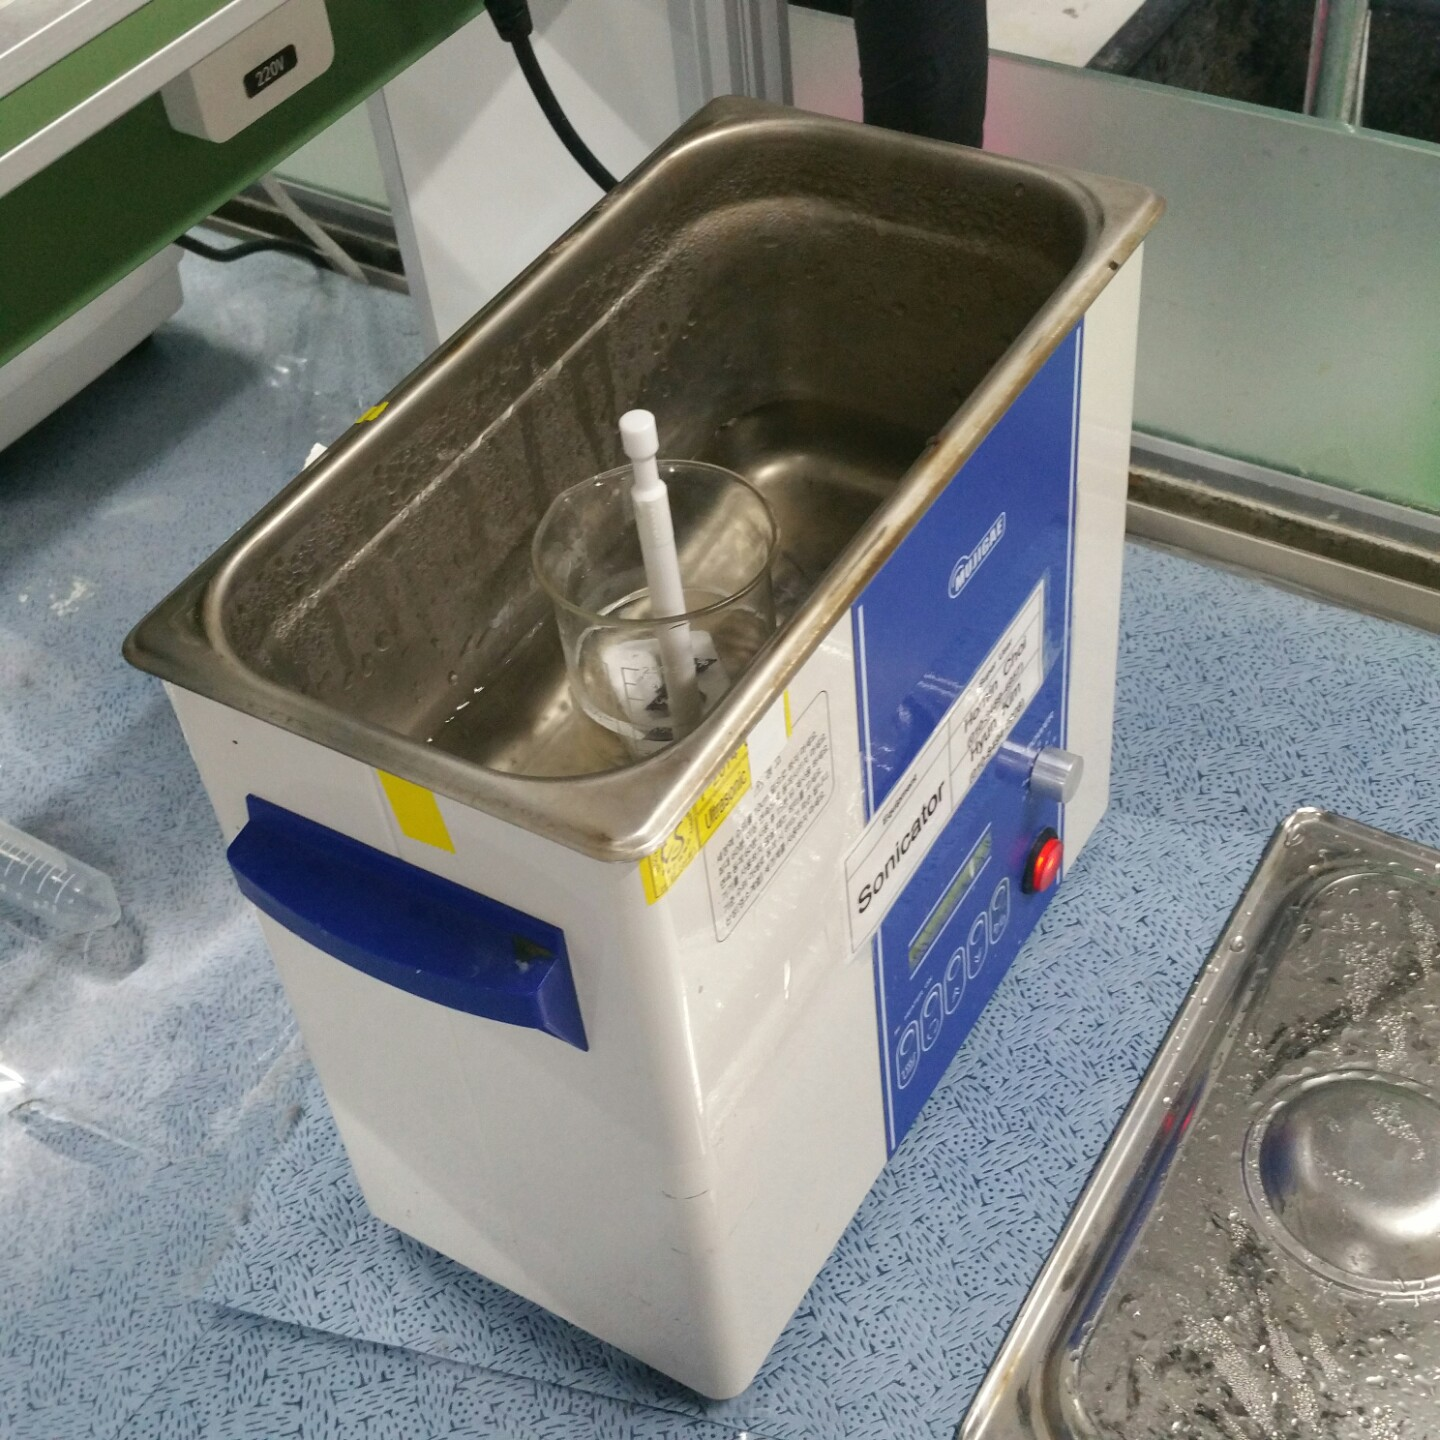
\includegraphics[width=0.3\textwidth]{sonicator}&
				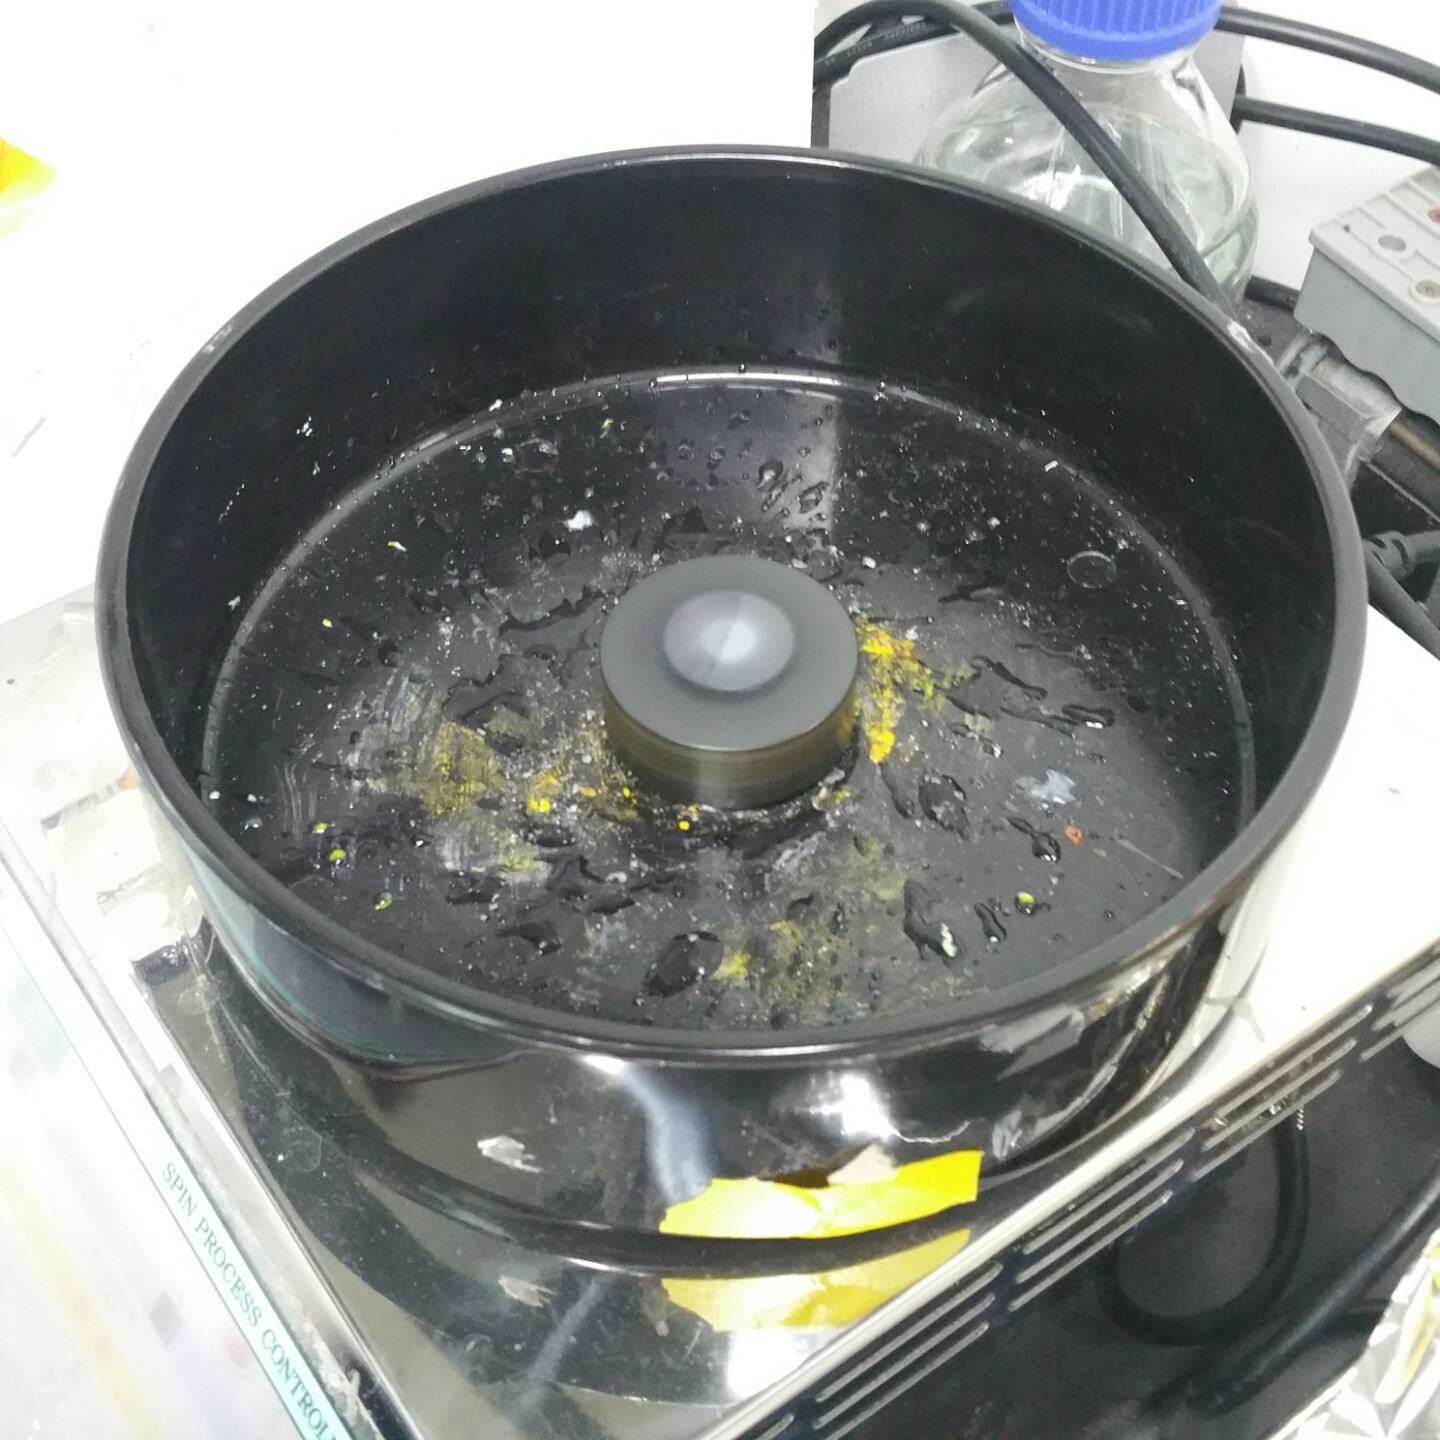
\includegraphics[width=0.3\textwidth]{spin_coating}&
				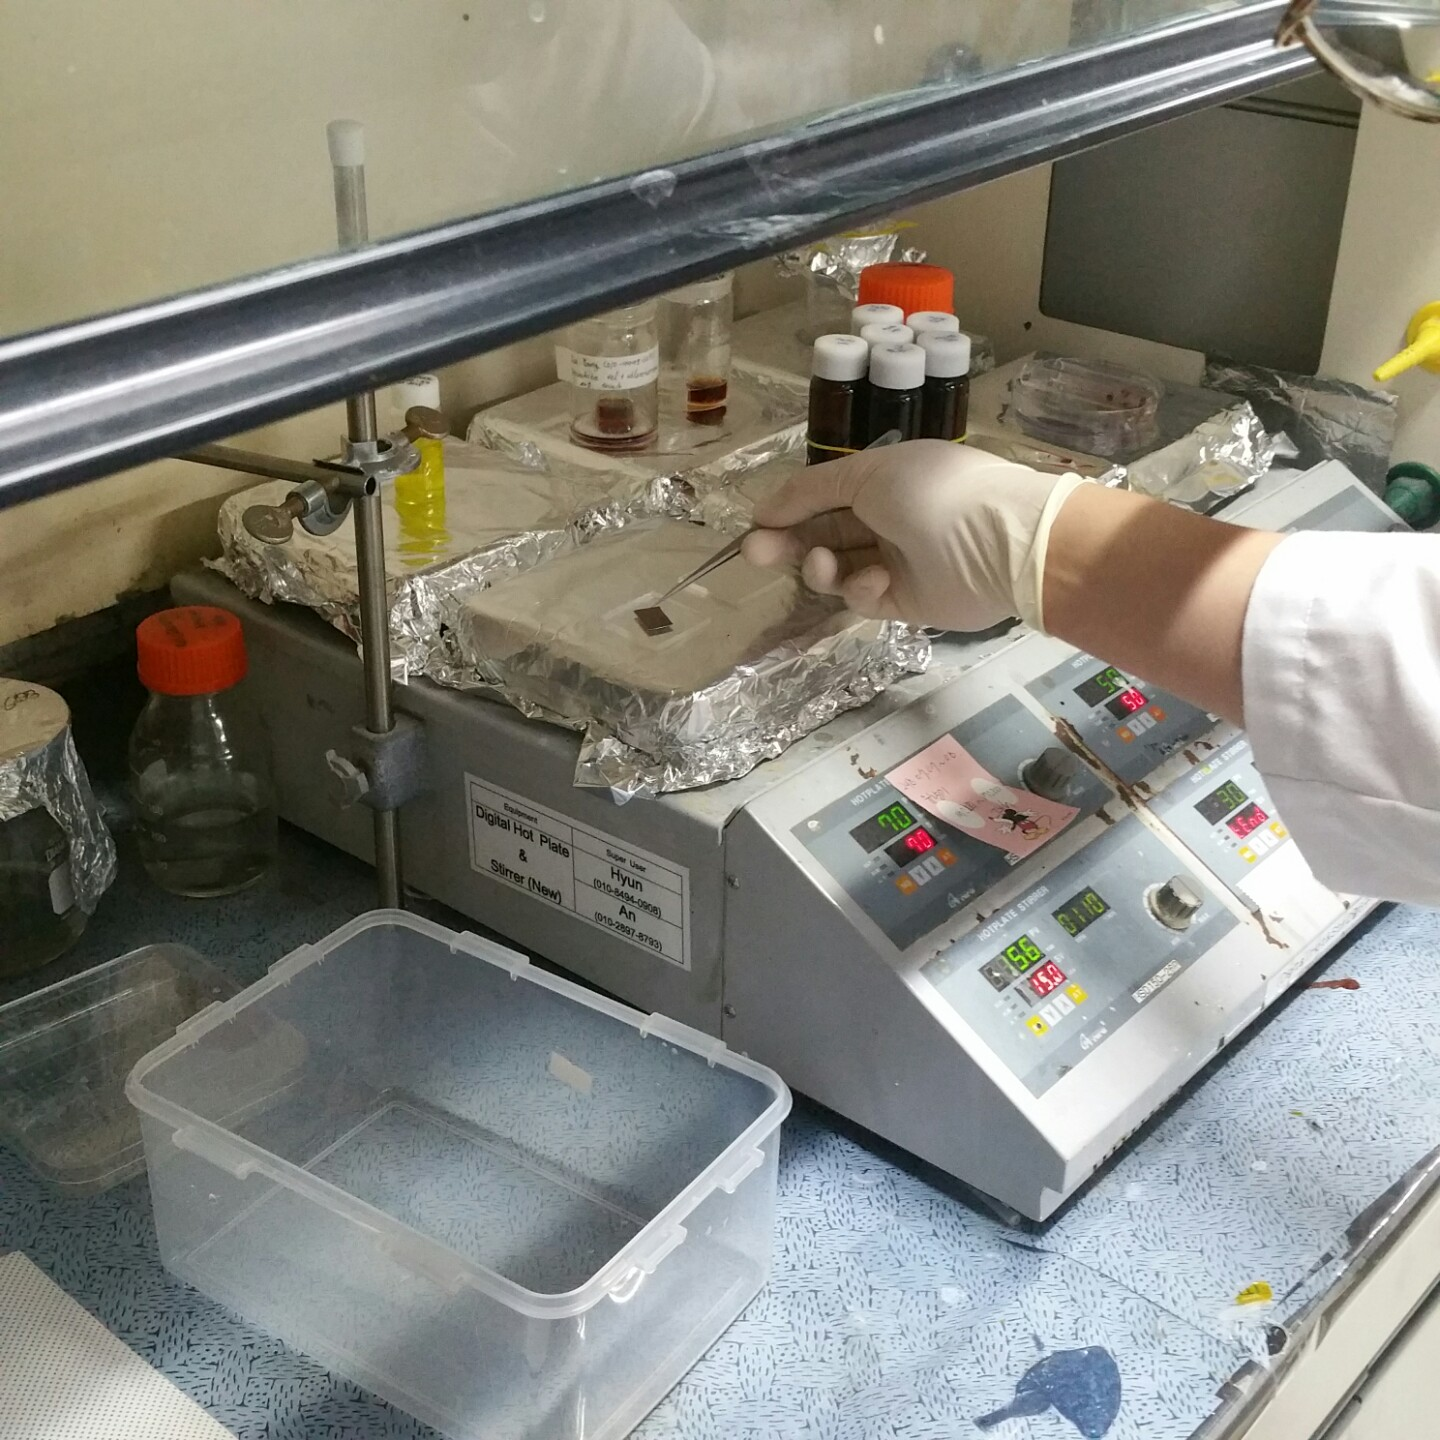
\includegraphics[width=0.3\textwidth]{hotplate}
			\end{tabular}
		\end{center}
		\begin{tikzpicture} [remember picture,overlay]
		\node[text=white] at (0.6, 4.7) {(a)};
		\node at (5.2, 4.7) {(b)};
		\node[text=white] at (10.1, 4.7) {(c)};
		\end{tikzpicture}	
		\caption{Sample production. (a) Sonicating, (b) Spin coating, (c) PDMS stamping on hot plate.}
		\label{fig:sample}  
	\end{figure}
	\item 결정이 생겼는지 광학현미경을 통해서 확인한 뒤(Figure 6), 가장 잘 형성된 결정에 405(nm) 파장의 레이저를 사용해서 PL 촬영을 진행하였다. 
	\begin{figure}[H]
		\begin{center}
			\begin{tabular}{cc}
				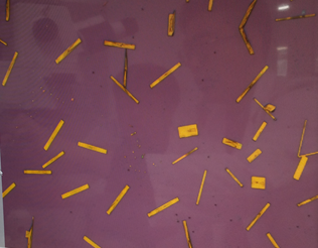
\includegraphics[width=0.45\textwidth]{OM}
			\end{tabular}
		\end{center}
		\caption{A silicon wafer taken with an OM (optical microscope).}
		\label{fig:om}  
	\end{figure}
\end{enumerate}
Perovskite는 70도 이상의 온도에서 빠른 degradation이 나타나는 것으로 알려져 있다. 본 실험에서는 100도에서 PDMS stamping을 진행하였는데 온도가 높아도 결정이 비교적 적게 생기긴 하지만 PL peak의 위치는 변하지 않기 때문에 그렇게 진행하였다.


\subsection{데이터 추출}
제작된 sample을 NT-MDT Spectrum Instruments 사의 Ntegra 기기를 통하여 $75(um)\times75(um)$의 영역을 PL mapping 하였다. 생성된 단결정에 측정할 위치를 정해 놓고 PL을 측정하였다.  PL mapping이란 특정 영역에서의 모든 PL 데이터를 얻는 기법으로 전체적인 특성을 한눈에 볼 수 있다는 장점이 있다. 이 데이터는 레이저의 조리개를 $OD = 2$ 로 맞춰놓은 ND2 상태에서 측정하였다. 이렇게 만들어진 파일에서는 임의의 점에서의 PL data를 얻어낼 수 있다는 장점이 있다.
\begin{figure}[H]
	\begin{center}
		\begin{tabular}{cc}
			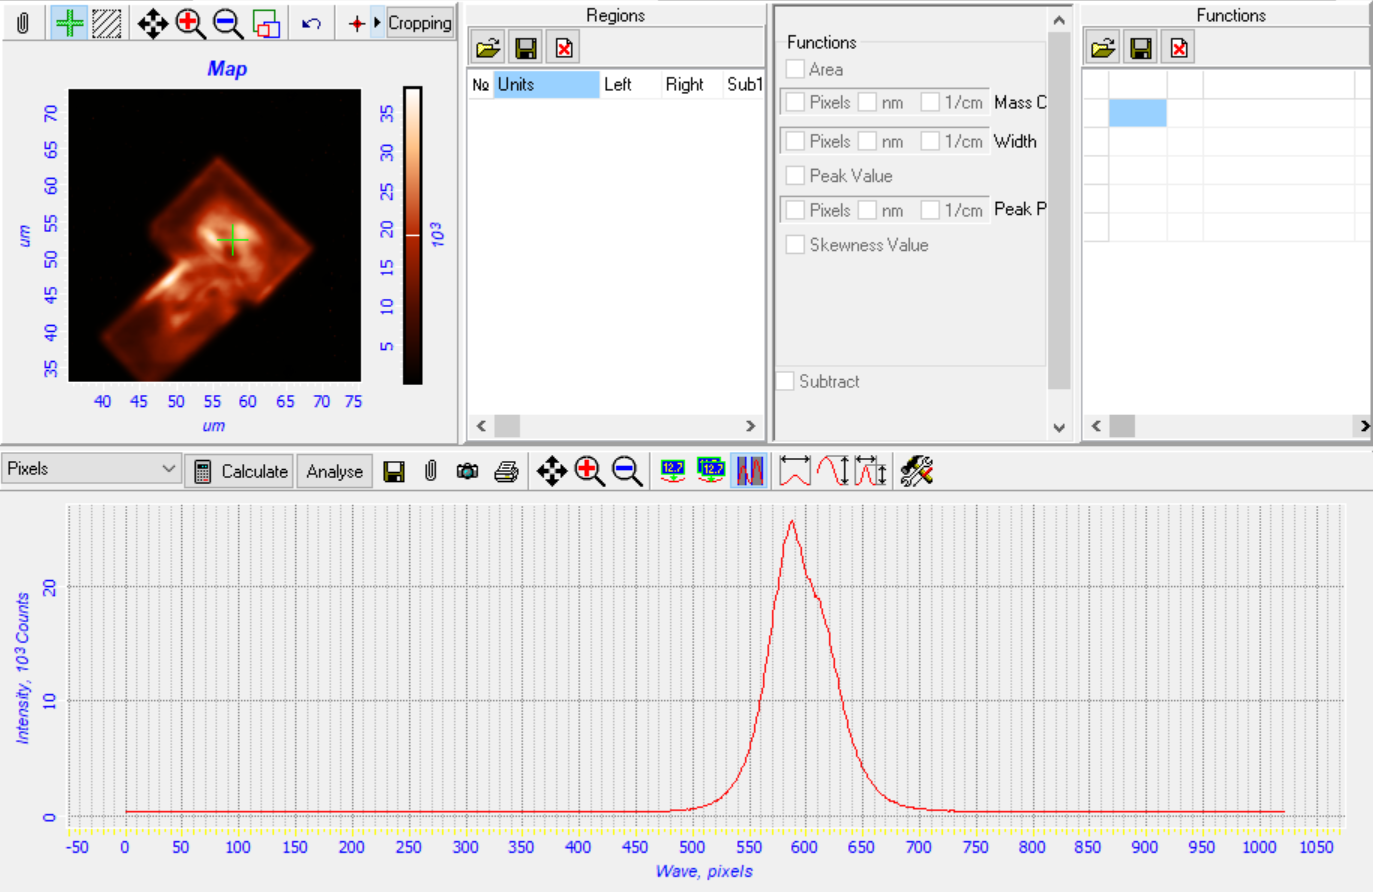
\includegraphics[width=0.65\textwidth]{Nova_screen_capture}&
			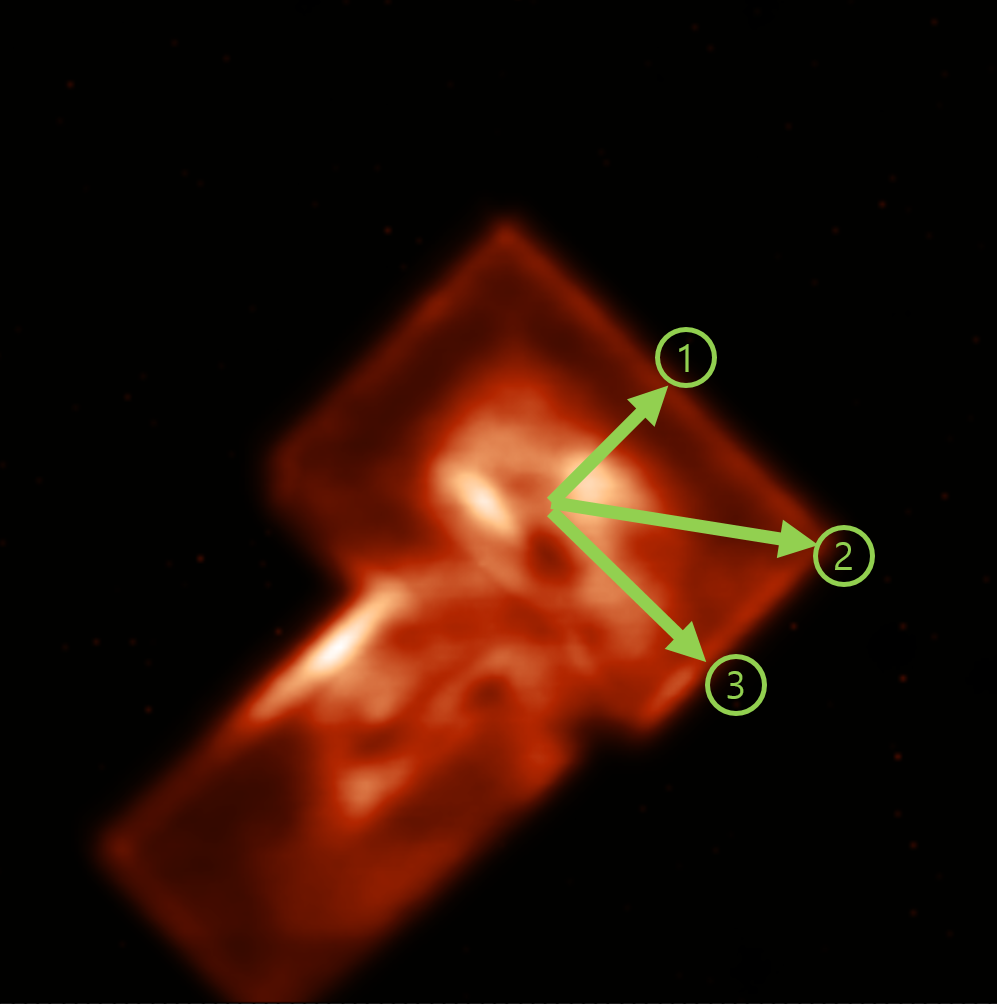
\includegraphics[width=0.4\textwidth]{line123}
		\end{tabular}
	\end{center}
	\begin{tikzpicture} [remember picture,overlay]
	\node at (0.6, 6.2) {(a)};
	\node[text=white] at (10.5, 6) {(b)};
	\end{tikzpicture}
	\caption{Extracting data and line setting. (a) Nova-Px program for extracting data, (b) line setting.}
	\label{fig:nova}  
\end{figure}
Nova Px 프로그램을 활용하여 PL mapping 된 파일에서 데이터를 각 점별로 뽑아내었다. Figure \ref{fig:nova}\와 같은 화면에서 십자의 위치를 조절하여 원하는 위치의 PL peak을 얻어낼 수 있다. 중앙에서부터 바깥으로 나갈 때의 PL peak의 경향성을 알아보기 위해 Figure \ref{fig:nova}의 오른쪽 사진에서 볼 수 있는 1, 2, 3 경로로 이동하며 PL peak 자료를 추출하였다.

Figure 7의 (b)에서 그림 상으로는 정중앙이 아닐 수 있지만, PL peak이 가장 높게 나온 곳이므로 올바른 경향성을 찾아내기 위하여 중앙을 대표하는 기준점으로 선정하였다. 기준점의 사진상 좌표는 (59.0, 53.6)이고, 선정된 기준점으로부터 바깥 방향으로 나가는 경로 1, 2, 3위의 관측점을 Table 1과 같이 설정하였다.

\begin{table}[H]%[width=1.0\linewidth]
	\caption{Routing lines 1, 2, and 3}
	\label{table01}
	\centering
	\begin{tabular}{c c}
	\toprule
	경로 번호 & 경로\\
	\toprule
	Line 1 & (59.0, 53.6, 33)-->(62.3, 56.9, 14) / (+0.4, +0.4) 씩 이동, 9개소 관측\\
	Line 2 & (59.0, 53.6, 33)-->(68.0, 51.3, 13) / (+0.8, -0.2) 씩 이동, 12개소 관측\\
	Line 3 & (59.0, 53.6, 33)-->(64.7, 47.9, 17) / (+0.4, -0.4) 씩 이동, 15개소 관측\\
	\toprule
	\end{tabular}
\end{table}
중앙으로 잡은 점을 point 0, 각 line에 대해 있는 점들을 point 1-1, 1-2, … , 1-8, 2-1, 2-2, … , 2-11, 3-1, 3-2, … , 3-14로 정의하였다. line 1은 point 0부터 point 1-8, line 2 은 point 0 부터 point 2-11, line 3은 point 0부터 point 3-14까지 이다. 
\\

\subsection{분석 과정}
\subsubsection{Point data peak fitting}
각 점의 추출된 data를 분석하기 위해서 Origin 9 프로그램을 사용하였다. Chen (2018) 에 의하면 $\rm CsPbBr_3$에서 biexciton과 exciton의 peak\이 나타나는 wave length\는 각각 약 580nm, 600nm 이다\cite{chen2018room}. 이 사실을 바탕으로 PL data에서 보인 peak\을 두 개의 peak의 합으로 fitting 하였다. Peak fitting\을 할 때 Hartley (1961)의 Gauss fitting 메커니즘을 프로그램에서 사용하였으며, biexciton 과 exciton이 존재하는 wavelength에 peak 위치를 설정한 후 fitting\을 진행하였다\cite{hartley1961modified}. Figure \ref{fig:point0}은 그중 하나의 예시이다.

\begin{figure}[H]
	\begin{center}
		\begin{tabular}{cc}
			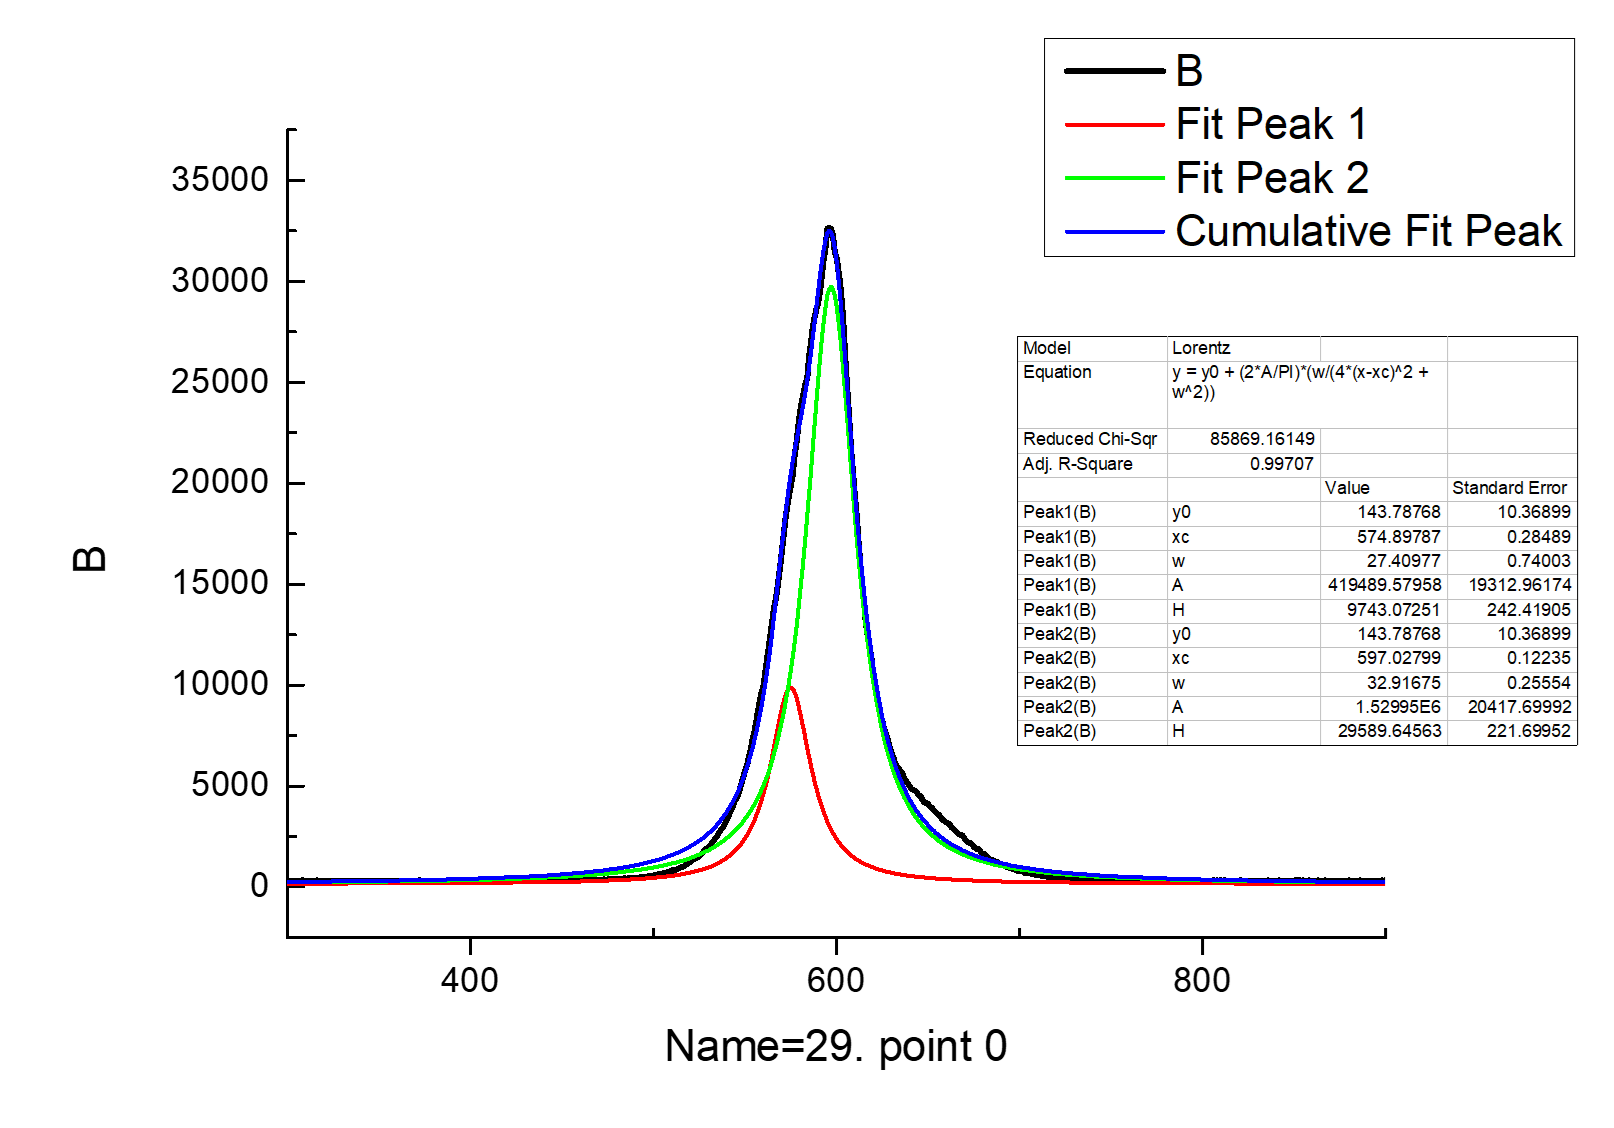
\includegraphics[width=0.8\textwidth]{point0}
		\end{tabular}
	\end{center}
	\caption{The PL data of the set point 0 is shown by sum of exciton and biexciton peak.}
	\label{fig:point0}  
\end{figure}

Figure \ref{fig:point0}\과 같이 multiple peak fitting을 마친 후에는 각 peak의 x값, 즉 wavelength 값과 y값, 즉 intensity 값을 데이터로 기록한 후 분석하였다.

\subsubsection{Line data analysis}
위의 과정에서 각 point 들의 data에 대한 peak fitting을 한 이후에 그 경향성을 보기 위해 필요한 과정이다. 분석하고자 하는 것은 중앙에서 바깥으로 가면서 peak intensity의 경향성이다. 이를 위해서 peak fitting 과정에서 얻은 데이터인 각 point에서의 biexciton, exciton peak의 intensity값을 y축, point 번호를 x 축으로 설정하여  line 1, line 2, line 3 별로 막대그래프를 그려서 경향성을 볼 수 있었다.
\\

\subsection{분석 결과 및 해석}
Line 1, Line 2, Line 3 에서의 결과를 각각 Figure \ref{fig:line1}, Figure \ref{fig:line2}, Figure \ref{fig:line3}에 나타내었다.

\begin{figure}[H]
	\begin{tabular}{cc}
		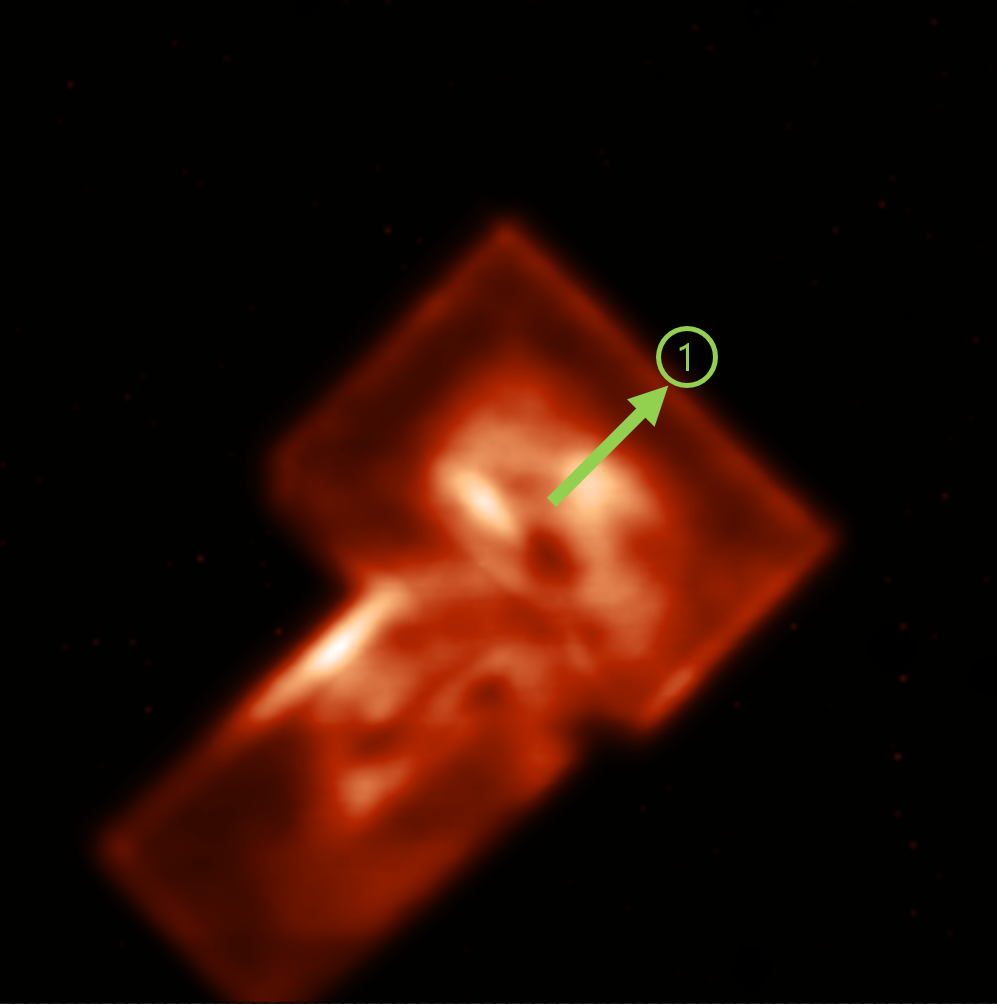
\includegraphics[width=0.3\textwidth]{line1}
		\begin{tikzpicture} [remember picture,overlay]	
		\node[text=white] at (-4, 4) {(a)};
		\end{tikzpicture}
		&
		\begin{tikzpicture}
		\begin{axis} [
		width=0.70\textwidth,%
		height = 5cm,%
		ybar,%
		bar width=5pt,
		title={Line 1},%
		xtick = data,%
		symbolic x coords={0, 1, 2, 3, 4, 5, 6, 7, 8},%
		xlabel= {Viewpoint},%
		ylabel= {Intensity(a.u.)},%
		ymin=0,ystep=5000,ymax=35000.0,%
		scaled y ticks = false,%
		ymajorgrids = true,
		legend style={at={(0.02,10)}},legend pos=north east]%
		\addplot table [x=no, y=biexciton] {./data/line1.csv}; %
		\addlegendentry {biexciton}%
		\addplot table [x=no, y=exciton] {./data/line1.csv}; %
		\addlegendentry {exciton}%
		\end{axis}
		\node at (-0.9, 3.5) {(b)};
		\end{tikzpicture}
	\end{tabular}
	\caption{(a) Route set to line 1, (b) Analyzed data :tendency in the path along line 1.}
	\label{fig:line1}  
\end{figure}




Figure \ref{fig:line1}, 즉 line 1에서는 exciton과 biexciton 모두 감소하는 추세를 보이다가 끝에서 증가하는 모습을 볼 수 있다.

\begin{figure}[H]
	\begin{tabular}{cc}
		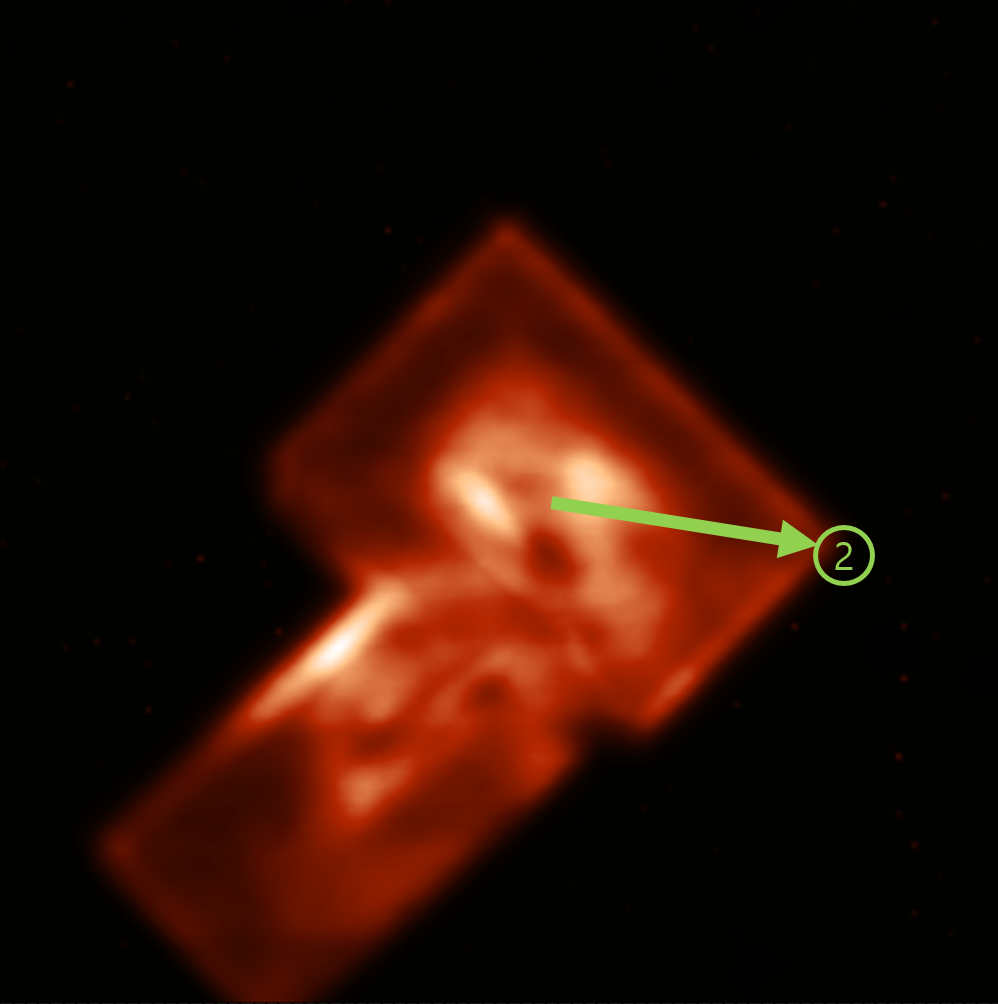
\includegraphics[width=0.3\textwidth]{line2}
		\begin{tikzpicture} [remember picture,overlay]	
		\node[text=white] at (-4, 4) {(a)};
		\end{tikzpicture}
		&
		\begin{tikzpicture}
		\begin{axis} [
		width=0.70\textwidth,%
		height = 5cm,%
		ybar,%
		bar width=5pt,
		title={Line 2},%
		xtick = data,%
		symbolic x coords={0, 1, 2, 3, 4, 5, 6, 7, 8, 9, 10, 11},%
		xlabel= {Viewpoint},%
		ylabel= {Intensity(a.u.)},%
		ymin=0,ystep=5000,ymax=35000.0,%
		scaled y ticks = false,%
		ymajorgrids = true,
		legend style={at={(0.02,10)}},legend pos=north east]%
		\addplot table [x=no, y=biexciton] {./data/line2.csv}; %
		\addlegendentry {biexciton}%
		\addplot table [x=no, y=exciton] {./data/line2.csv}; %
		\addlegendentry {exciton}%
		\end{axis}
		\node at (-0.9, 3.5) {(b)};
		\end{tikzpicture}
	\end{tabular}
	\caption{(a) shows the route set to line 2. (b)  is the analyzed data and shows the tendency in the path along line 2.}
	\label{fig:line2}  
\end{figure}


Figure \ref{fig:line2}, 즉 line 2에서는 exciton과 biexciton 모두 감소하는 추세를 보이다가 가장 끝 두점에서는 biexciton은 급격히 증가, exciton은 급격히 감소함을 볼 수 있다.

\begin{figure}[H]
	\begin{tabular}{cc}
		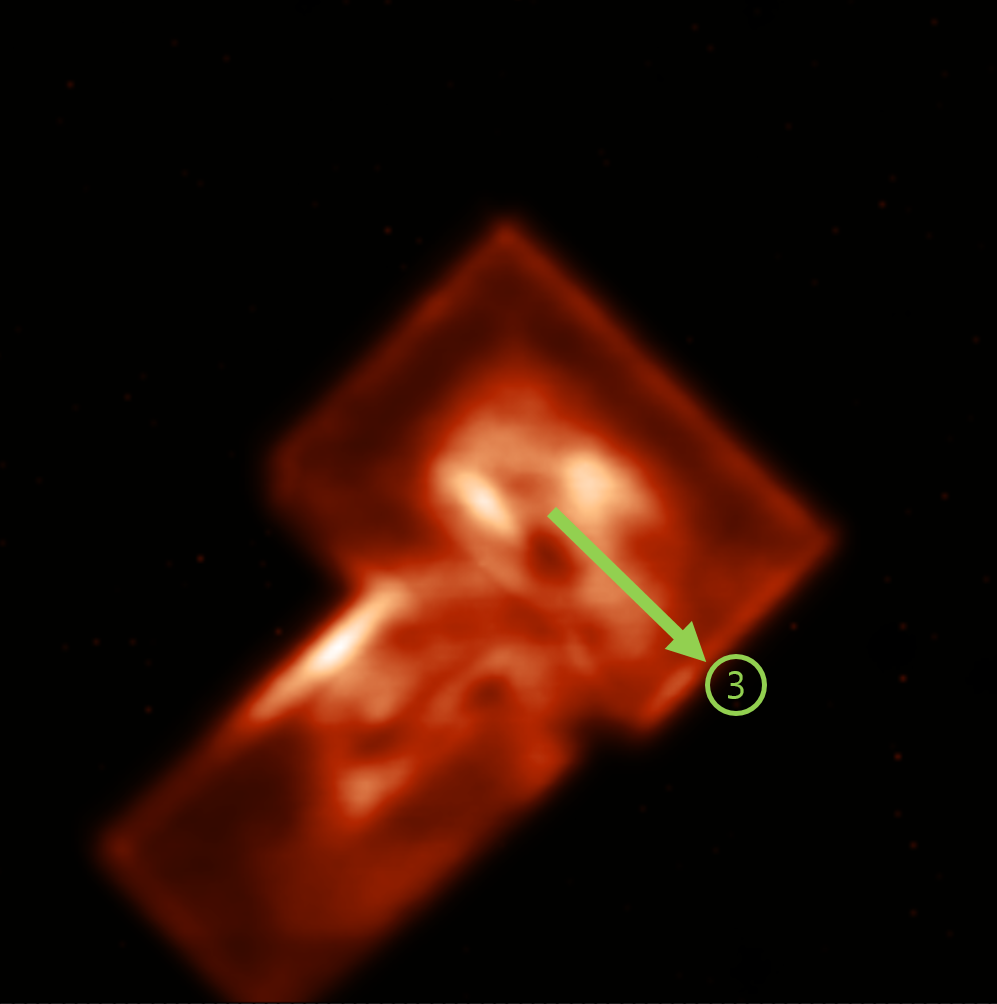
\includegraphics[width=0.3\textwidth]{line3}
		\begin{tikzpicture} [remember picture,overlay]	
		\node[text=white] at (-4, 4) {(a)};
		\end{tikzpicture}
		&
		\begin{tikzpicture}
		\begin{axis} [
		width=0.70\textwidth,%
		height = 5cm,%
		ybar,%
		bar width=5pt,
		title={Line 3},%
		xtick = data,%
		symbolic x coords={0, 1, 2, 3, 4, 5, 6, 7, 8, 9, 10, 11, 12, 13, 14},%
		xlabel= {Viewpoint},%
		ylabel= {Intensity(a.u.)},%
		ymin=0,ystep=5000,ymax=35000.0,%
		scaled y ticks = false,%
		ymajorgrids = true,
		legend style={at={(0.02,10)}},legend pos=north east]%
		\addplot table [x=no, y=biexciton] {./data/line3.csv}; %
		\addlegendentry {biexciton}%
		\addplot table [x=no, y=exciton] {./data/line3.csv}; %
		\addlegendentry {exciton}%
		\end{axis}
		\node at (-0.9, 3.5) {(b)};
		\end{tikzpicture}
	\end{tabular}
	\caption{(a) shows the route set to line 3. (b)  is the analyzed data and shows the tendency in the path along line 3.}
	\label{fig:line3}  
\end{figure}





Figure \ref{fig:line3}, 즉 line 3에서는 exciton은 감소, biexciton은 증가하는 추세를 보이다가 가장 끝 두 점에서는 biexciton은 급격히 감소, exciton은 급격히 증가함을 볼 수 있다.

세 line에서 exciton, biexciton 각각의 공통되는 경향성이나 규칙은 찾아보기 어렵다. 하지만 중앙에서 중간까지 갈 때는 특정한 경향성을 보이는 듯하다가 가장 바깥, 가장자리에서 그 경향성이 반대되는 모습을 볼 수 있다. 종합적으로 보았을 때는 가장자리로 가면서 감소하는 모습을 보이다가 다시 증가하는 모습이 세 line 모두에서 나타났다.

같은 ND2로 찍은 PL 데이터를 관찰했을 때, 완전한 가장자리를 제외하면 바깥으로 갈수록 biexciton peak의 상대적인 세기가 세짐을 관찰할 수 있었다. 

PL 측정 시 $\rm CsPbBr_3$가 구조상의 deformation이 일어나지 않으므로 비슷한 양의 carrier가 전도띠로 가는 것은 자명하다. 이 carrier들은 각각 exciton이나 biexciton의 형태로 존재하게 되는데, PL에서 biexciton에 의한 peak가 더 우세하게 관찰된 것이라고 해석할 수 있다.


	 와 같이 작성
	%%%% 주의
	%%%% 파일이 나뉠 때마다 자동으로 페이지넘김(\clearpage)가 됩니다. 
	%%%% 따라서 subsection을 나누는 용도로는 사용하지 마십시오.
	%%%% \include{sub/experiment} 와 같이...
	
	%-----------------------------------------------------
%  Introduction
%-----------------------------------------------------

\section{서론}
\subsection{연구 동기}

페로브스카이트(Perovskite) 구조를 가지고 있는 결정에 레이저를 쏘았을 때 Figure \ref{fig:waveguide} 에서 볼 수 있듯이 빛이 결정의 바깥쪽으로 퍼지는 현상을 관찰할 수 있었고, waveguiding effect에 의한 현상으로 추정하였다. Waveguiding effect\는 굴절률 차이에 의한 경로 변경이나 에너지 출입의 메커니즘에 의해서 빛이 특정 장소로 모이는 현상을 뜻한다. Yarita (2017)의 연구와 같이 페로브스카이트의 구조, 광학적 특성을 분석한 실험에서는 XRD(X-ray diffraction), TRPL(Time-Resolved Photoluminescence), PL(Photoluminescence) 등 여러 가지 장비를 이용하여 분석을 하였지만 중심으로부터 가장자리까지의 경향성을 분석하는 것은 없었다\cite{yarita2017dynamics}. 특히 PL 분석에서는 PL로 찍었을 때 나오는 개형의 half width\과 peak에 대해 분석하였지만, 그것을 통해 waveguiding effect의 명확한 원인은 찾지 못하였다. 본 논문에서는 그 원인을 명확히 파악하고자 PL data\를 exciton peak과 biexciton peak에 대해서 따로 분석하였다. 

\begin{figure}[H]
	\begin{center}
			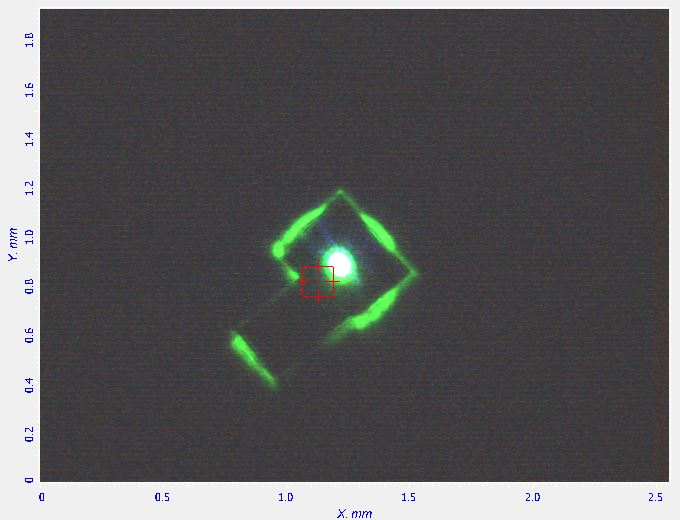
\includegraphics[width=0.6\textwidth]{waveguiding_effect}
	\end{center}
	\caption{Appearance of $\rm CsPbBr3$ single crystal when laser is shot on it.}
	\label{fig:waveguide}  
\end{figure}

\subsection{이론적 배경}

\subsubsection{Perovskite}
Green et al.(2014)에 의하면 페로브스카이트는 L. A. Perovski의 이름을 따서 명명된 물질로, 처음 발견된 $\rm CaTiO_3$  같은 구조를 가진 결정을 통틀어서 부르는 말이을\cite{green2014emergence}. 일반적으로 $\rm ABX_3$로 쓰며, Figure 2와 같은 결정구조를 가지고 있다. 여기서 A와 M에는 여러 금속 양이온들이 해당되고, X에는 보통 16족, 17족 음이온들이 해당된다.


\begin{figure}[H]
	\begin{center}
			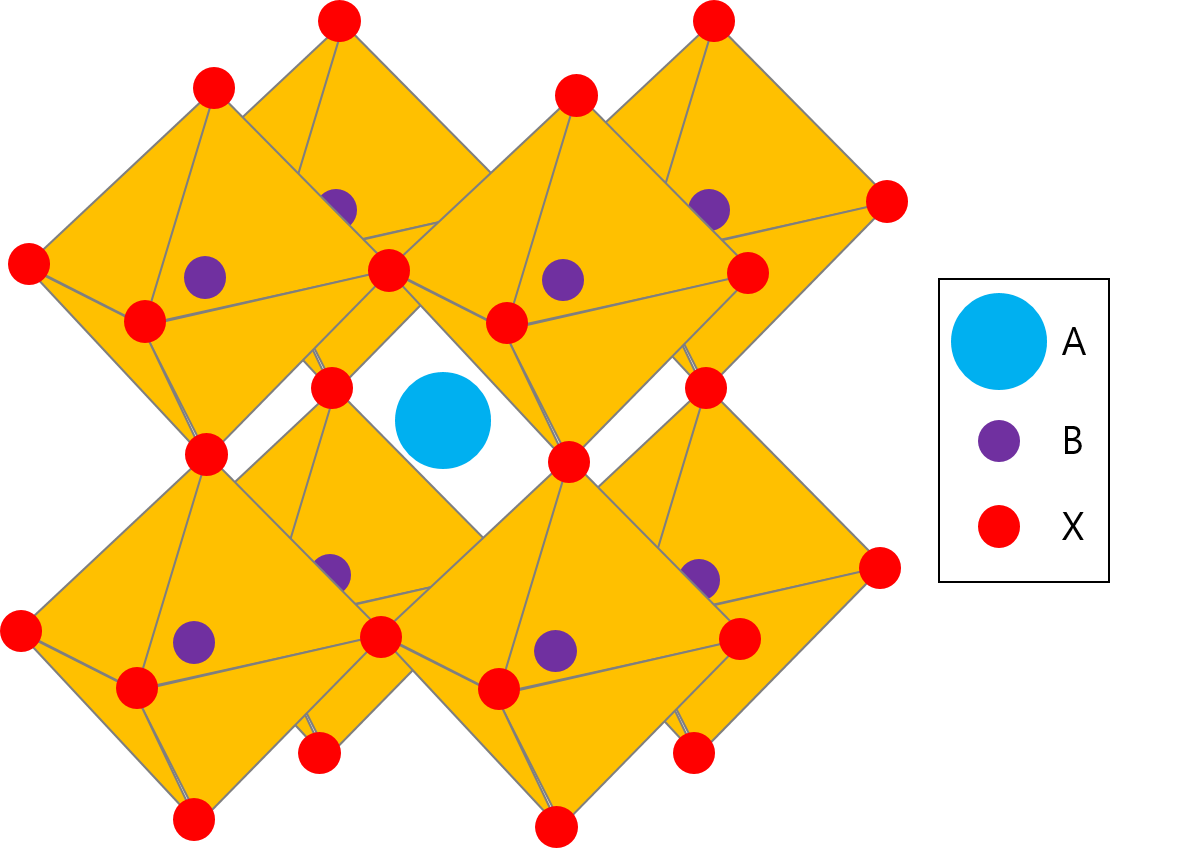
\includegraphics[width=0.6\textwidth]{perovskite}
	\end{center}
	\caption{Basic structure of perovskite.}
	\label{fig:perov} 
\end{figure}

A 위치에는 금속뿐만 아니라 유기물인  methylammonium $\rm(CH_3NH_3^+)$이나 ethylammonium $\rm(CH_3CH_2NH_3^+)$를 넣어 페로브스카이트를 구성할 수 있다. Green et al.(2014)에 의하면 쇼트키-퀘이서 효율 한계(Shockley Queisser Efficiency Limit)에 의해 물질의 밴드갭에 따라 전지 효율의 이론적 최댓값이 존재한다\cite{green2014emergence}. 페로브스카이트는 각 자리에 여러 물질을 바꿔 넣을 수 있으므로 이론적인 최대 효율 값에 비슷하게 도달할 수 있는 장점이 있다. 이 뿐만 아니라 가능한 밴드갭 영역이 넓고 꼭짓점을 공유하는 팔면체들의 회로망 덕분에 캐리어의 이동성이 좋아서 전하가 잘 수송되기도 한다\cite{green2014emergence}.

또, 페로브스카이트는 합성 과정이 간단하며 태양 빛을 잘 흡수하기 때문에 각광받고 있으며, 이와 관련되어 여러 연구가 진행되고 있다. Huang(2009)에 의하면 페로브스카이트가 결정 상태가 아닐 때에는 defect가 존재하여 물성을 탐색할 때 정확하지 못하다는 문제를 해결하기 위해서 단결정을 제작멶면하였다\cite{huang2009fabrication}. 본 연구에서는 단결정을 제작하는 새로운 방식 중 하나인 PDMS(Polydimethylsiloxane) stamping을 이용하여 단결정을 제작하였다.
\\

\subsubsection{Photoluminescence}

\begin{figure}[H]
	\begin{center}
			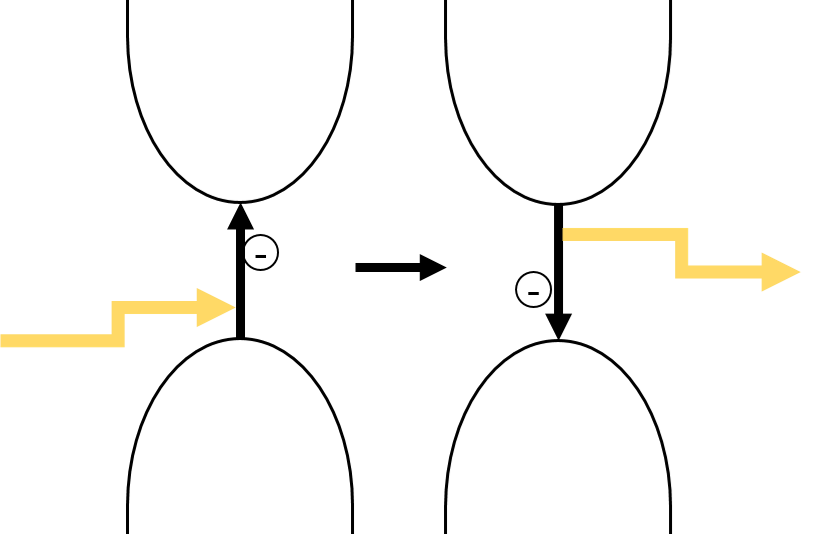
\includegraphics[width=0.8\textwidth]{PL}
	\end{center}
	\caption{Energy released from the relaxation process of excited electrons.}
	\label{fig:pl} 
\end{figure}

PL은 광자를 통해 에너지를 흡수한 물질이 그 에너지를 다시 방출하는 것을 이르는 것이다. 이론적으로는 넣어준 빛의 파장과 동일한 파장의 빛이 방출되지만, 실제로는 에너지가 더 낮은, 파장이 더 긴 빛이 방출된다. 

빛이 방출되는 과정은 크게 photoexcitation, relaxation, radiative recombination의 세 가지 과정으로 나뉜다. photoexcitation은 외부에서 주어진 빛에 의해 전자가 들뜨는 현상을 이르는 것이고 relaxation은 들뜬 전자가 전도띠에서 에너지가 가장 낮은 부분으로, 정공이 원자 띠에서 에너지가 가장 높은 부분으로 이동하는 과정이다. 마지막으로 radiative recombination 과정은 Figure \ref{fig:pl}\과 같이 들뜬 전자가 다시 정공과 결합하는 과정을 의미한다. 이때 방출되는 빛의 파장별 intensity를 PL로 측정하여 data\를 얻을 수 있다.
\\

\subsubsection{Exciton, biexciton의 의미}
\begin{figure}[H]
	\begin{center}
			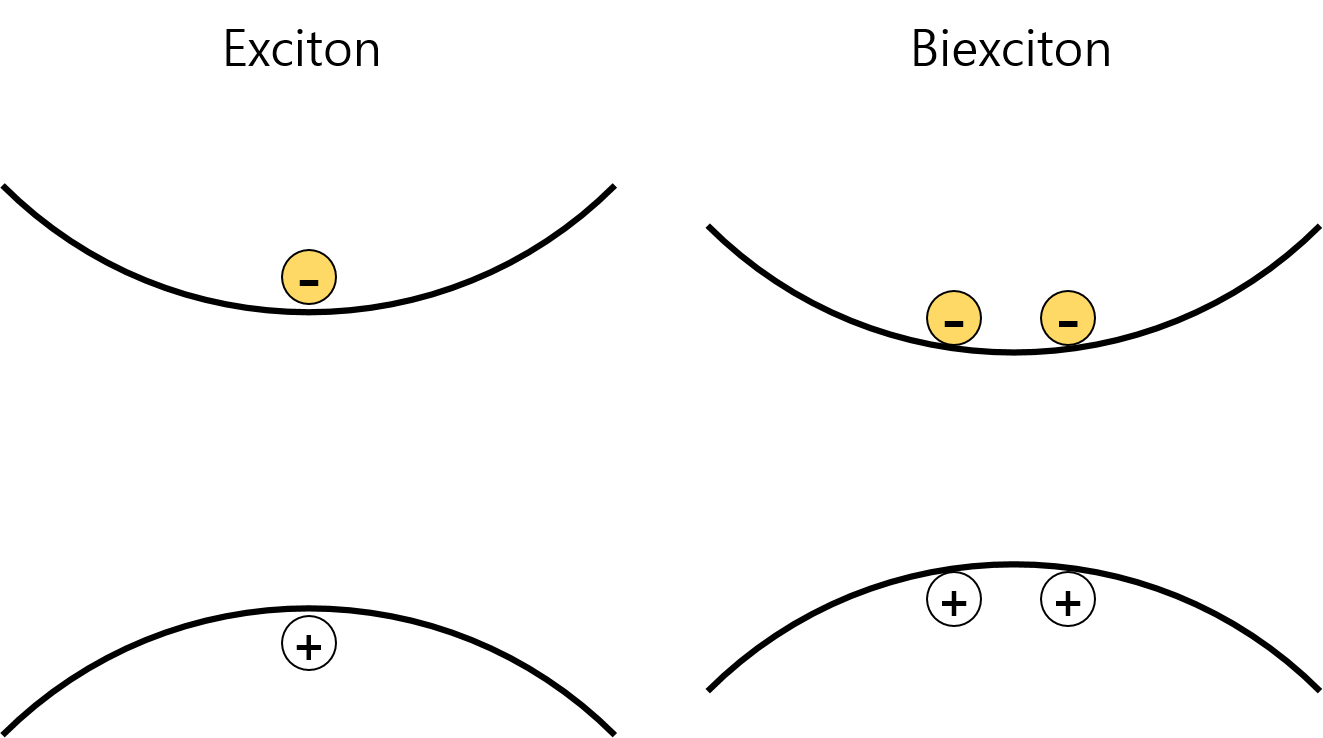
\includegraphics[width=0.6\textwidth]{exciton_biexciton}
	\end{center}
	\caption{Image of exciton and biexciton.}
	\label{fig:ex}  
\end{figure}
Figure \ref{fig:ex}에서 볼 수 있듯이 exciton은 PL 측정 과정에서 양공과 전자 하나의 쌍을 말하며, 이것이 두 개가 쌍을 이루고 있을 때 그것을 biexciton이라 칭한다. Triexciton 또한 존재하지만 그 존재 빈도가 극히 낮아서 스펙트럼에 나타나지 않는다. 
\\
\subsubsection{Waveguiding effect}
Waveguiding effect란 도파관 효과로, 빛이나 에너지가 여러 가지 이유에 의해서 특정 지점으로 모이거나 빛의 경로가 조절되는 현상을 말한다. 가장 기본적인 예시로 빛이 전반사되는 광섬유가 있다. J.Valenta (2002), Jin (1999)의 연구를 보면 광결정에서 에너지의 이득을 보기 위해서 발생하는 waveguiding effect가 존재한다\cite{valenta2002waveguiding} \cite{jin1999band}. 


\subsubsection{ND filter}
ND(Neutral Density) filter에 특정한 파장대의 빛을 투과시키면 세기가 감소하는 특성이 있다. 이는 강한 레이저 빛이 광학기구에 직접 닿으면 센서나 광학 기구가 손상될 수 있기 때문에 사용한다. 투과율 T는 OD(Optical Density)값으로 정의되며 편의에 의해 OD값에 따라 ND filter 표기는 식 \ref{eq:002}\와 같이 결정된다.
\begin{equation}
T(\%)~=~10^{-OD}~\times~100
\label{eq:002}
\end{equation}
\\
\subsection{연구 목적 및 연구 문제}
본 연구에 앞서 수행한 연구에서는 XRD, TRPL, PL을 통해 단결정 페로브스카이트의 구조적, 광학적 특성을 분석하였다. XRD는 성공적이었으나 위치별로 분석한 PL 분석에서는 스펙트럼이 비대칭적으로 나타났음에도 불구하고 peak와 half width로만 분석했기에 경향성을 분석할 때에 exciton peak 와 biexciton peak의 합의 경향성을 볼 수 있었다. 하지만 결정 내부의 radiative recombination에서 방출되는 빛의 defect와 결정의 순도에 관한 것은 두 가지 peak을 따로 분석해야 알 수 있다. Chen(2018)은 exciton과 biexciton을 따로 생각하고 온도에 따른 exciton과 biexciton peak의 변화를 분석하였고, 본 연구에서는 이를 참고하였다 \cite{chen2018room}. 

본 연구는 PL 분석 시에 나타나는 peak의 exciton, biexciton별 분석을 통하여 wave guiding effect의 원인을 분석하는 것이 목적이다. wave guiding effect\와 전자의 photoluminescence\와의 연관성을 찾기 위해 위치에 따른 exciton, biexciton peak의 intensity를 조사하고 경향성을 분석한다.

본 연구에서 제시하는 연구 문제는 다음과 같다:
\begin{enumerate}
	\item $\rm CsPbBr_3$ 단결정에 레이저를 쏘았을 때 바깥쪽에서 그 빛이 나타나는 것은 wave guiding effect에 의한 것인가?
	\item Wave guiding effect에 의한 효과라면 전자의 photoluminescence와는 어떤 관련이 있는가? 
\end{enumerate}

 % Introduction
	\section{연구 과정 및 결과}

\subsection{샘플 제작}
본 연구에서는 간단하고 빠르게 페로브스카이트 결정을 만들 수 있는 PDMS stamping 방법을 사용하였다. 다음은 PDMS stamping 방법으로 페로브스카이트 결정 샘플을 제작하는 과정이다.
\begin{enumerate}
	\item $\rm CsPbBr_3$을 만들기 위해 $\rm CsBr$과 $\rm PbBr_2$를 1:1의 몰 비율로 섞고 용매는 DMSO(Dimethyl Sulfoxide)를 사용하였다.
	\item Sonication을 이용해서 용매와 용질을 균일하게 섞어주었다.
	\item Silicon wafer 위에 제조된 용액을 스포이트를 이용해서 떨어뜨린 뒤, 2,000rpm으로 1분간 회전시키는 spin coating을 이용하여 균일하게 펼쳐주었다.
	\item 섭씨 100도로 달궈놓은 핫플레이트에서 silicon wafer를 5분간 PDMS로 눌러주었다.
	\begin{figure}[H]
		\begin{center}
			\begin{tabular}{ccc}
				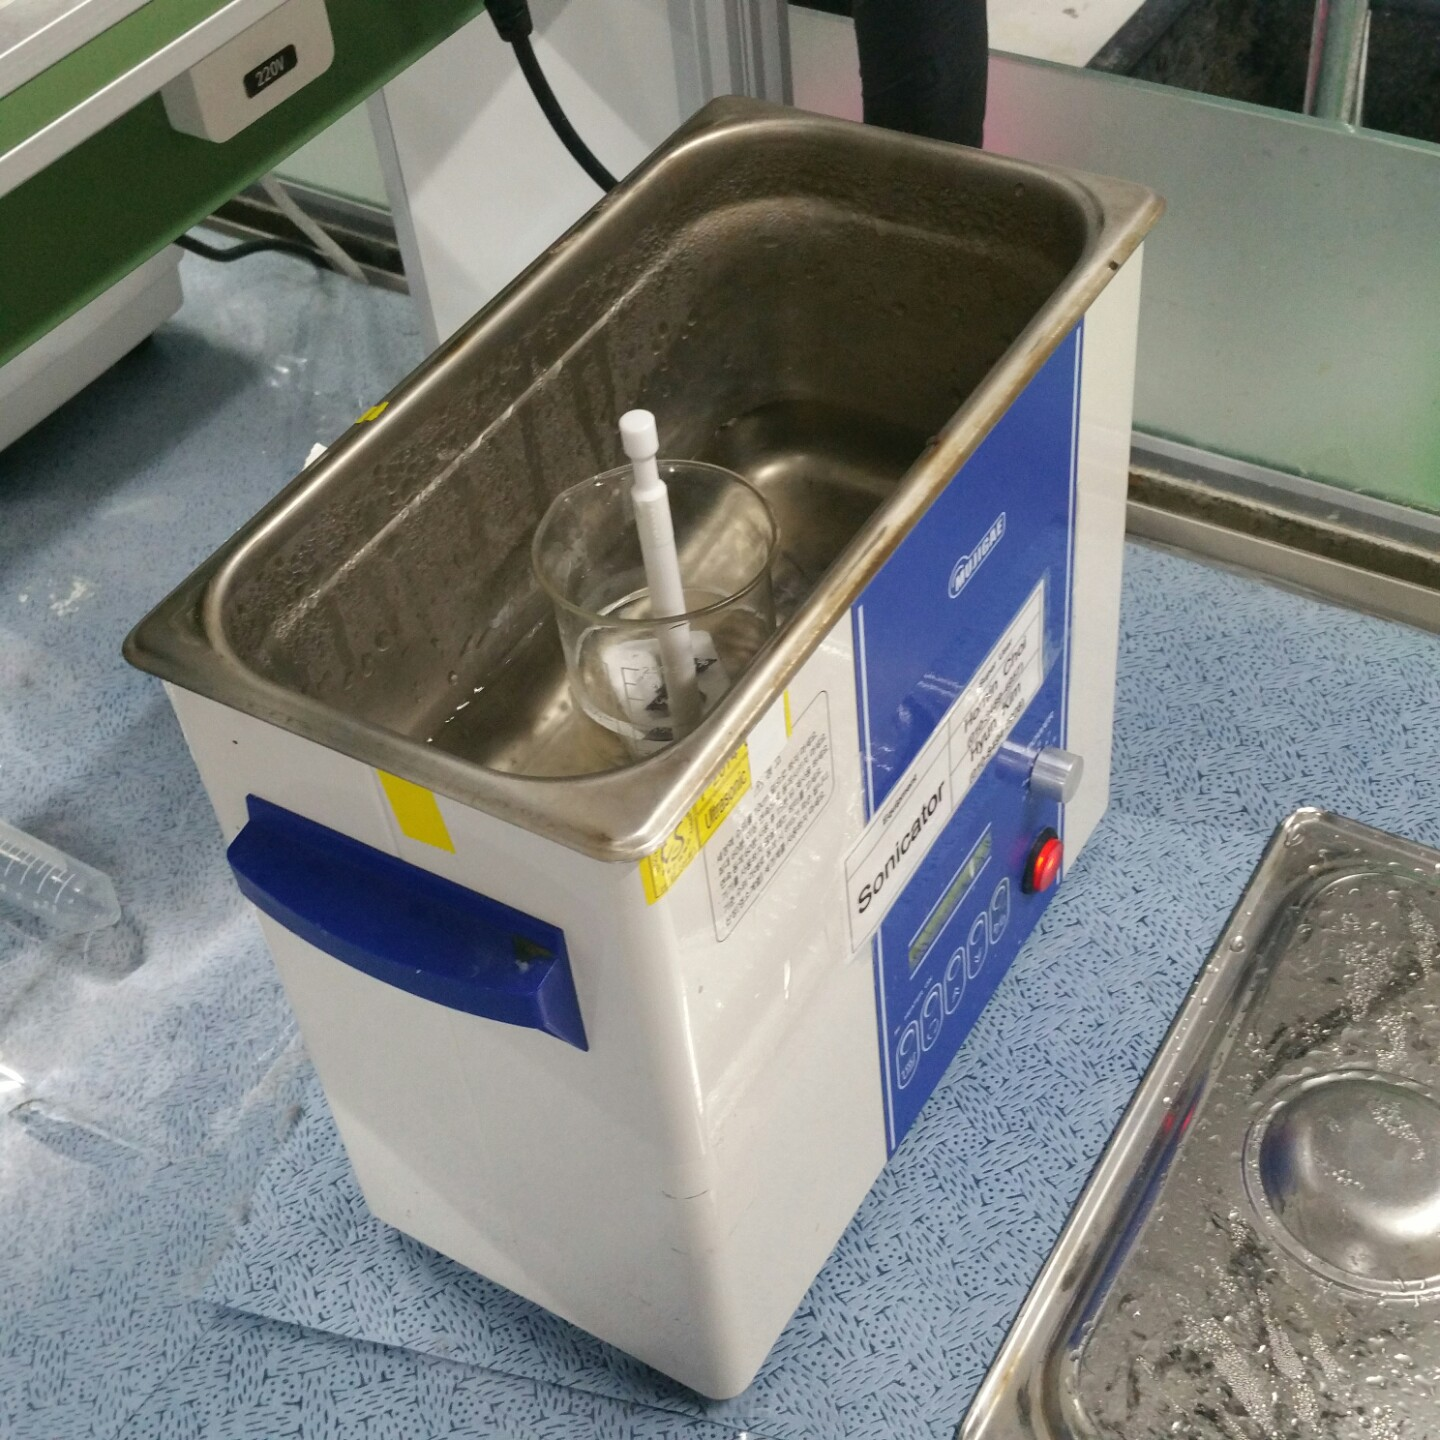
\includegraphics[width=0.3\textwidth]{sonicator}&
				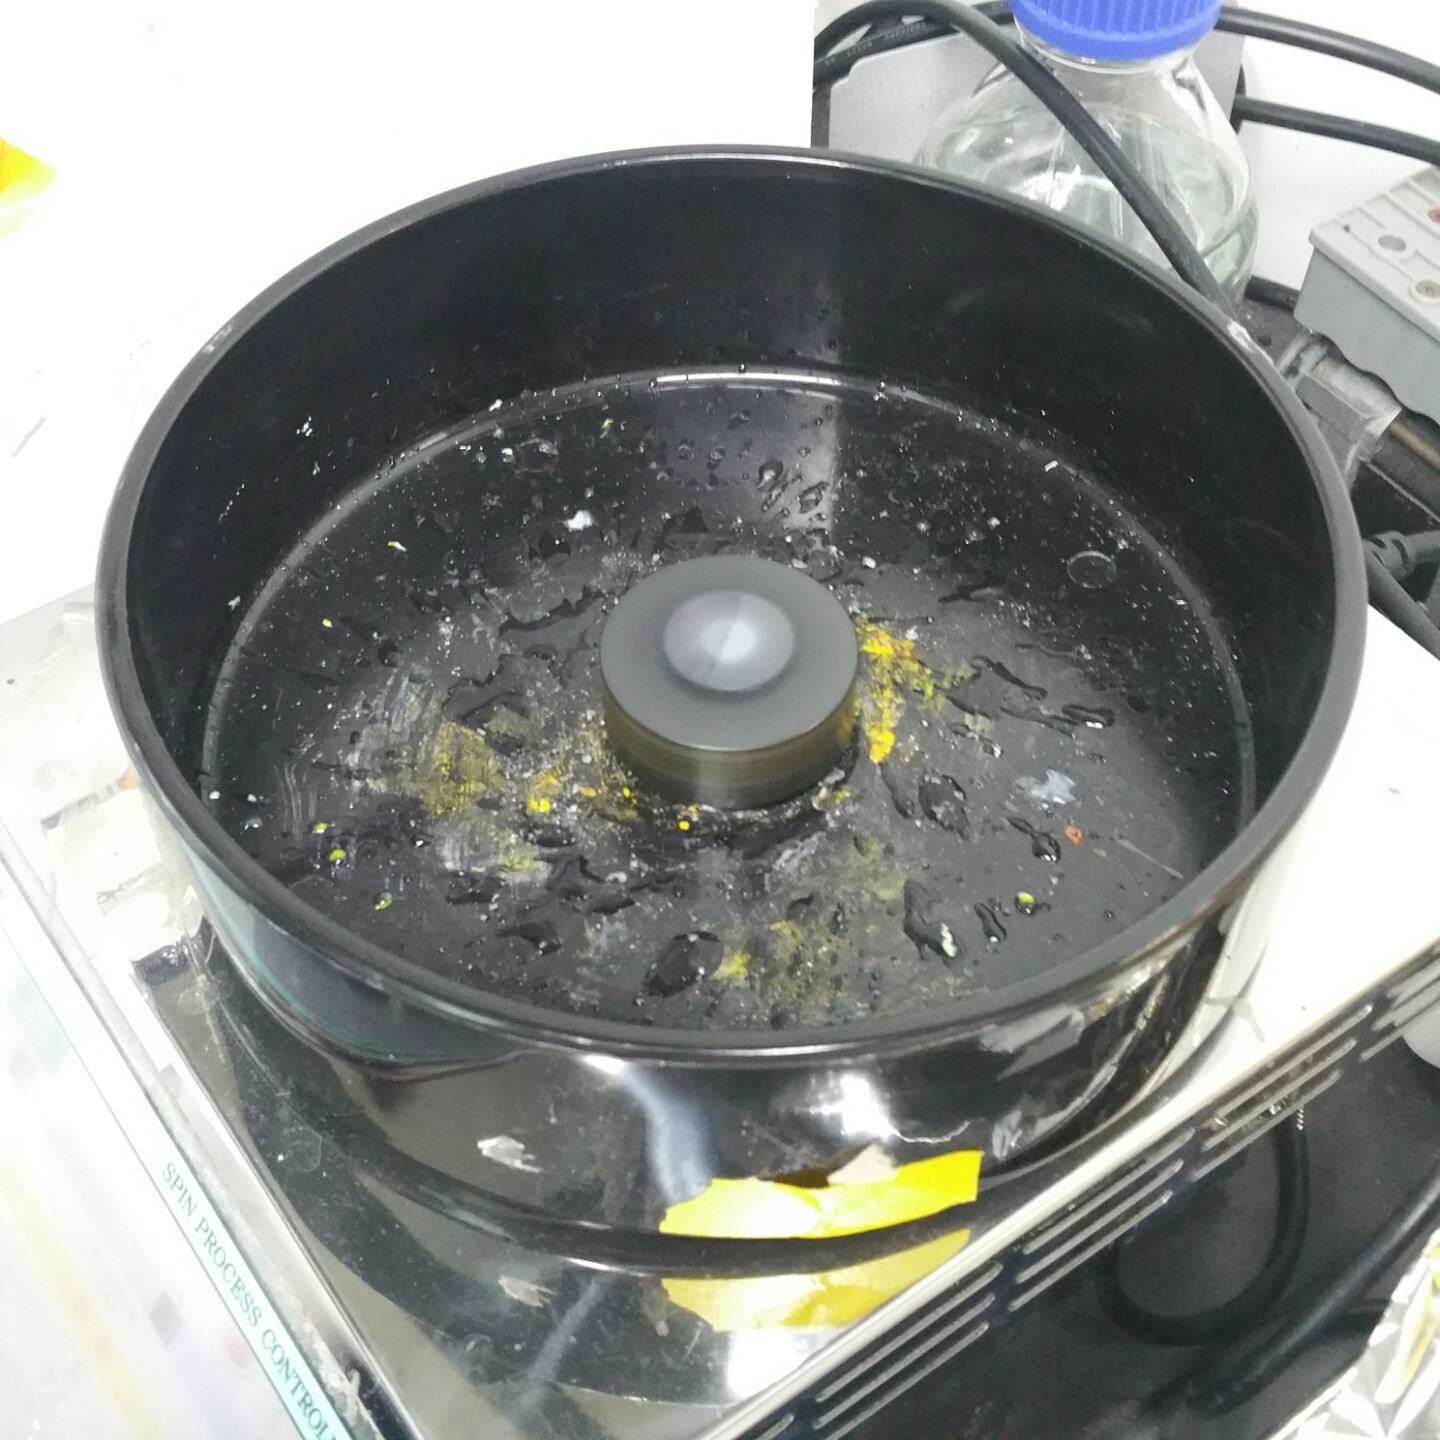
\includegraphics[width=0.3\textwidth]{spin_coating}&
				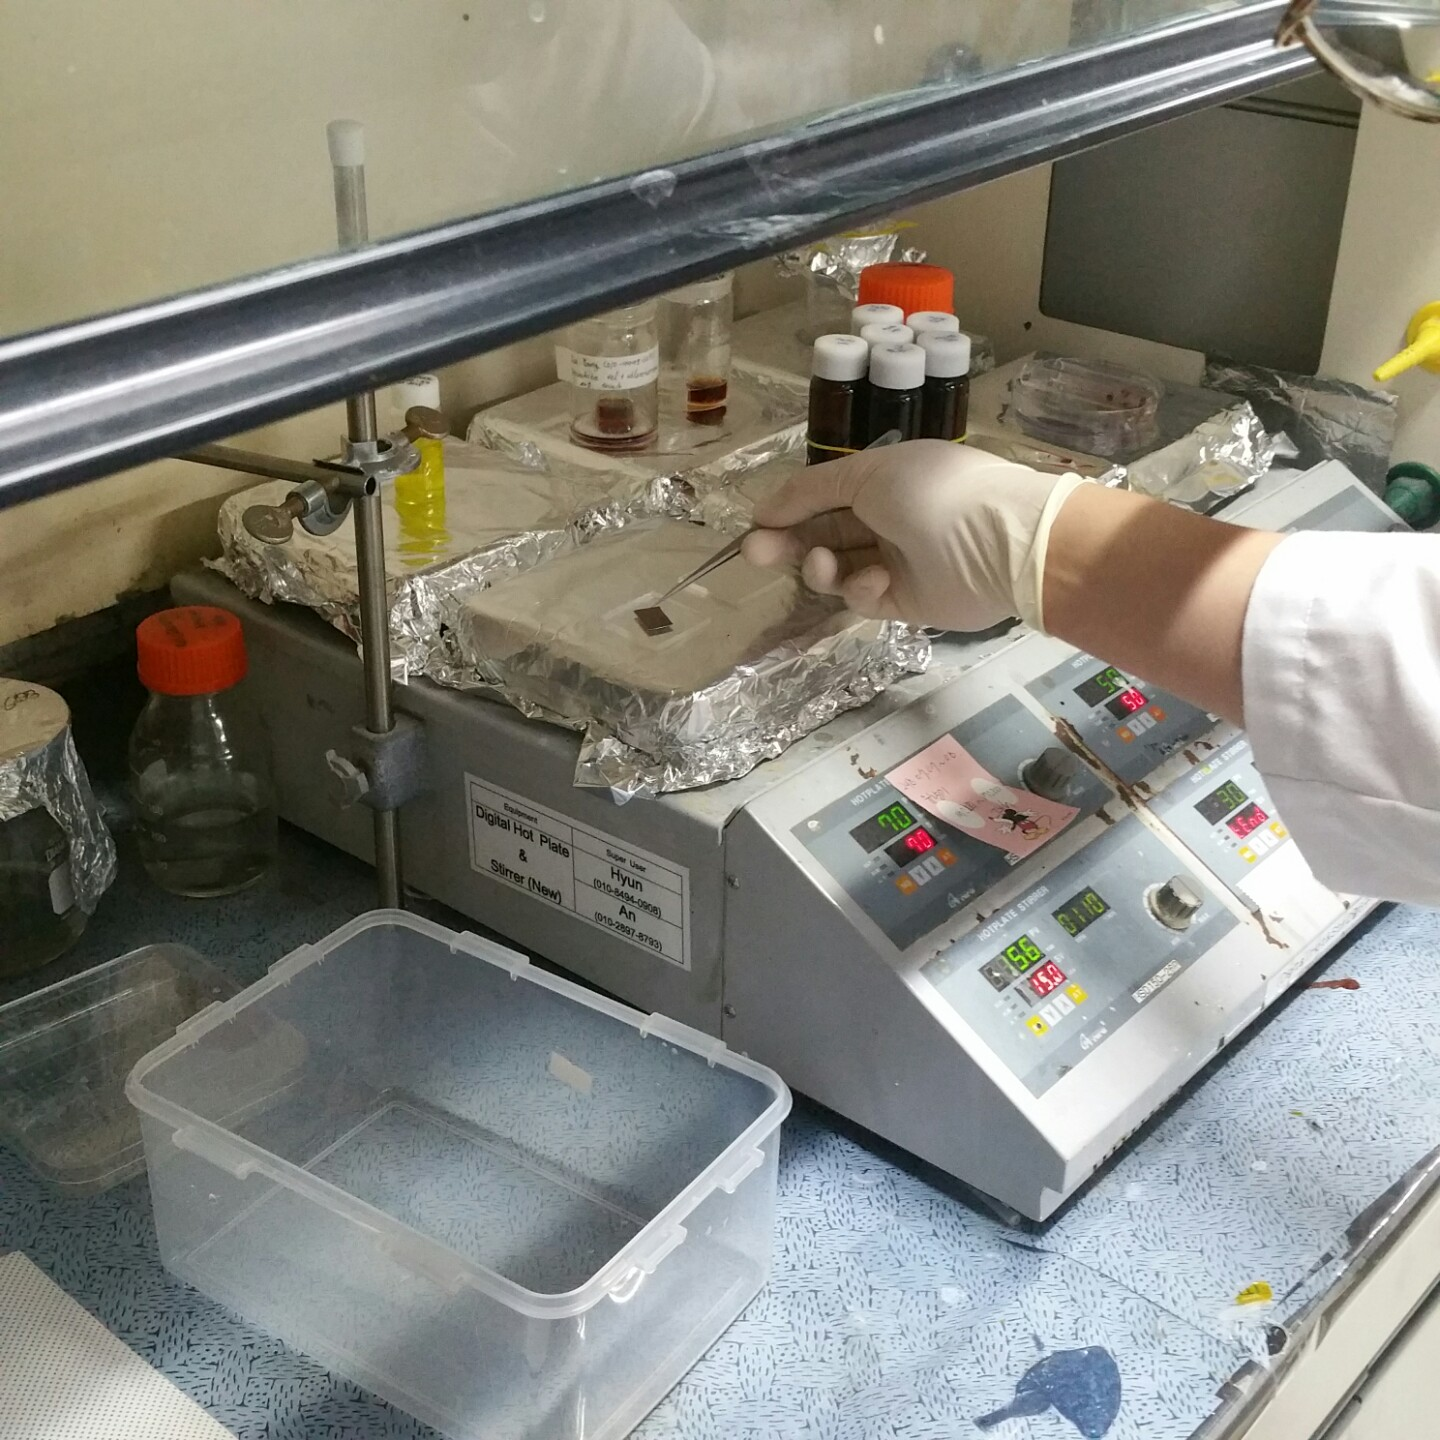
\includegraphics[width=0.3\textwidth]{hotplate}
			\end{tabular}
		\end{center}
		\begin{tikzpicture} [remember picture,overlay]
		\node[text=white] at (0.6, 4.7) {(a)};
		\node at (5.2, 4.7) {(b)};
		\node[text=white] at (10.1, 4.7) {(c)};
		\end{tikzpicture}	
		\caption{Sample production. (a) Sonicating, (b) Spin coating, (c) PDMS stamping on hot plate.}
		\label{fig:sample}  
	\end{figure}
	\item 결정이 생겼는지 광학현미경을 통해서 확인한 뒤(Figure 6), 가장 잘 형성된 결정에 405(nm) 파장의 레이저를 사용해서 PL 촬영을 진행하였다. 
	\begin{figure}[H]
		\begin{center}
			\begin{tabular}{cc}
				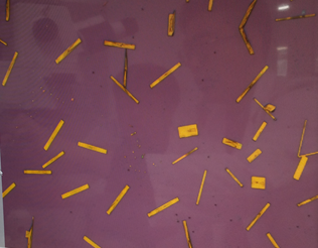
\includegraphics[width=0.45\textwidth]{OM}
			\end{tabular}
		\end{center}
		\caption{A silicon wafer taken with an OM (optical microscope).}
		\label{fig:om}  
	\end{figure}
\end{enumerate}
Perovskite는 70도 이상의 온도에서 빠른 degradation이 나타나는 것으로 알려져 있다. 본 실험에서는 100도에서 PDMS stamping을 진행하였는데 온도가 높아도 결정이 비교적 적게 생기긴 하지만 PL peak의 위치는 변하지 않기 때문에 그렇게 진행하였다.


\subsection{데이터 추출}
제작된 sample을 NT-MDT Spectrum Instruments 사의 Ntegra 기기를 통하여 $75(um)\times75(um)$의 영역을 PL mapping 하였다. 생성된 단결정에 측정할 위치를 정해 놓고 PL을 측정하였다.  PL mapping이란 특정 영역에서의 모든 PL 데이터를 얻는 기법으로 전체적인 특성을 한눈에 볼 수 있다는 장점이 있다. 이 데이터는 레이저의 조리개를 $OD = 2$ 로 맞춰놓은 ND2 상태에서 측정하였다. 이렇게 만들어진 파일에서는 임의의 점에서의 PL data를 얻어낼 수 있다는 장점이 있다.
\begin{figure}[H]
	\begin{center}
		\begin{tabular}{cc}
			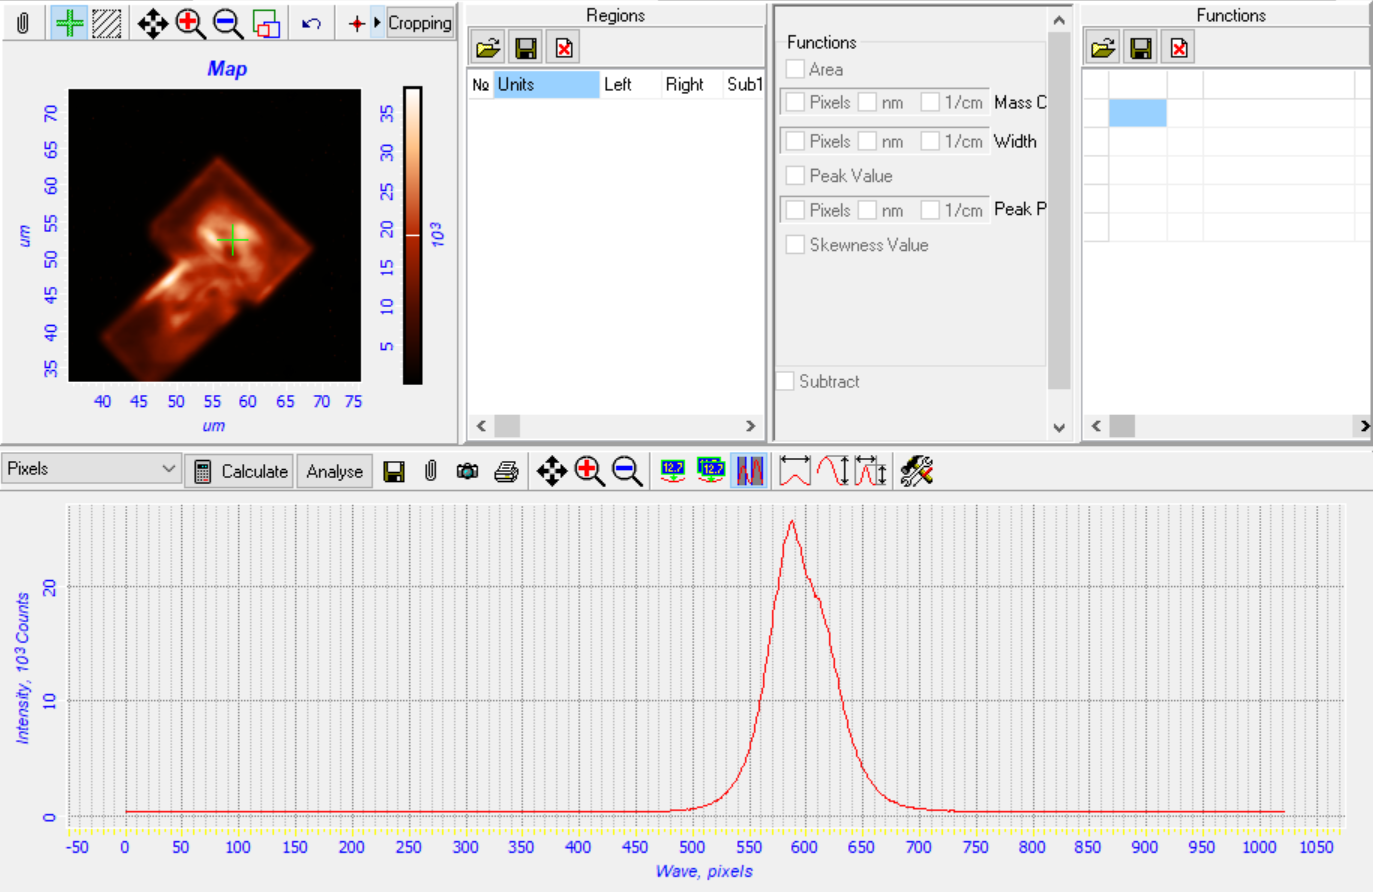
\includegraphics[width=0.65\textwidth]{Nova_screen_capture}&
			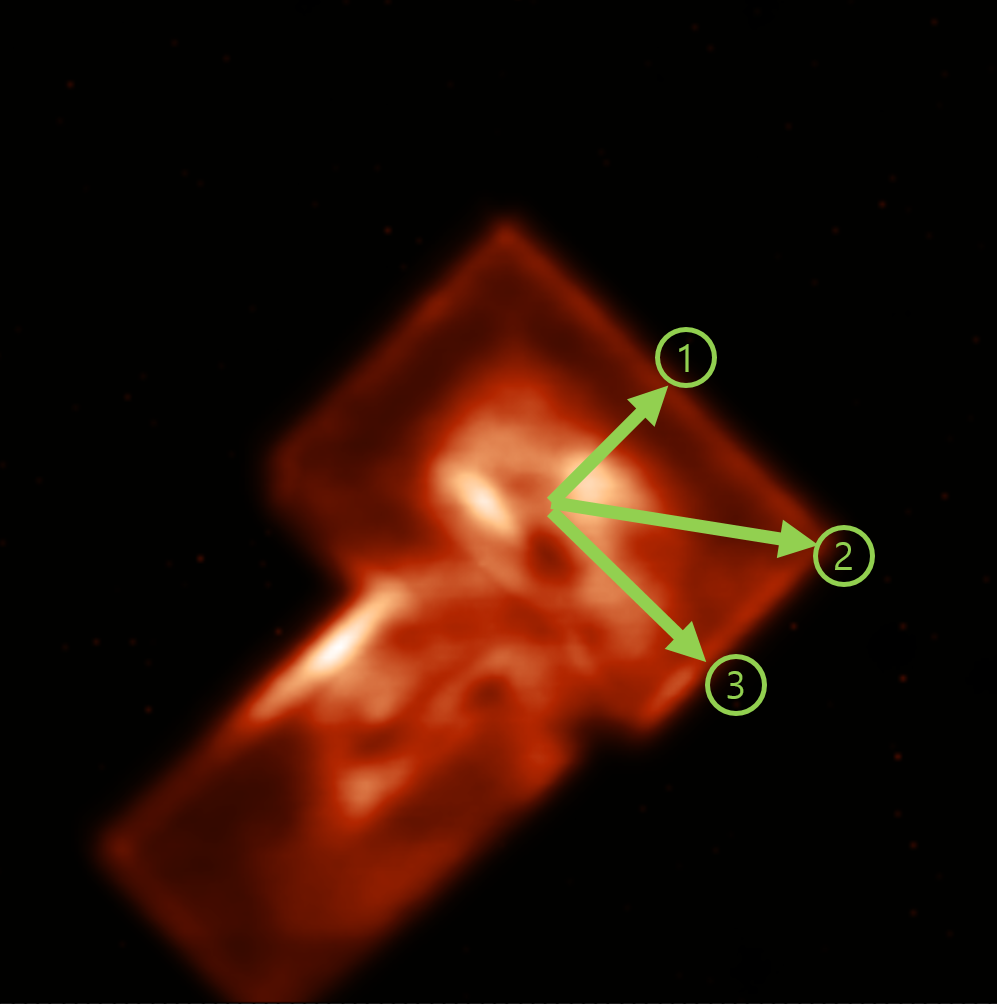
\includegraphics[width=0.4\textwidth]{line123}
		\end{tabular}
	\end{center}
	\begin{tikzpicture} [remember picture,overlay]
	\node at (0.6, 6.2) {(a)};
	\node[text=white] at (10.5, 6) {(b)};
	\end{tikzpicture}
	\caption{Extracting data and line setting. (a) Nova-Px program for extracting data, (b) line setting.}
	\label{fig:nova}  
\end{figure}
Nova Px 프로그램을 활용하여 PL mapping 된 파일에서 데이터를 각 점별로 뽑아내었다. Figure \ref{fig:nova}\와 같은 화면에서 십자의 위치를 조절하여 원하는 위치의 PL peak을 얻어낼 수 있다. 중앙에서부터 바깥으로 나갈 때의 PL peak의 경향성을 알아보기 위해 Figure \ref{fig:nova}의 오른쪽 사진에서 볼 수 있는 1, 2, 3 경로로 이동하며 PL peak 자료를 추출하였다.

Figure 7의 (b)에서 그림 상으로는 정중앙이 아닐 수 있지만, PL peak이 가장 높게 나온 곳이므로 올바른 경향성을 찾아내기 위하여 중앙을 대표하는 기준점으로 선정하였다. 기준점의 사진상 좌표는 (59.0, 53.6)이고, 선정된 기준점으로부터 바깥 방향으로 나가는 경로 1, 2, 3위의 관측점을 Table 1과 같이 설정하였다.

\begin{table}[H]%[width=1.0\linewidth]
	\caption{Routing lines 1, 2, and 3}
	\label{table01}
	\centering
	\begin{tabular}{c c}
	\toprule
	경로 번호 & 경로\\
	\toprule
	Line 1 & (59.0, 53.6, 33)-->(62.3, 56.9, 14) / (+0.4, +0.4) 씩 이동, 9개소 관측\\
	Line 2 & (59.0, 53.6, 33)-->(68.0, 51.3, 13) / (+0.8, -0.2) 씩 이동, 12개소 관측\\
	Line 3 & (59.0, 53.6, 33)-->(64.7, 47.9, 17) / (+0.4, -0.4) 씩 이동, 15개소 관측\\
	\toprule
	\end{tabular}
\end{table}
중앙으로 잡은 점을 point 0, 각 line에 대해 있는 점들을 point 1-1, 1-2, … , 1-8, 2-1, 2-2, … , 2-11, 3-1, 3-2, … , 3-14로 정의하였다. line 1은 point 0부터 point 1-8, line 2 은 point 0 부터 point 2-11, line 3은 point 0부터 point 3-14까지 이다. 
\\

\subsection{분석 과정}
\subsubsection{Point data peak fitting}
각 점의 추출된 data를 분석하기 위해서 Origin 9 프로그램을 사용하였다. Chen (2018) 에 의하면 $\rm CsPbBr_3$에서 biexciton과 exciton의 peak\이 나타나는 wave length\는 각각 약 580nm, 600nm 이다\cite{chen2018room}. 이 사실을 바탕으로 PL data에서 보인 peak\을 두 개의 peak의 합으로 fitting 하였다. Peak fitting\을 할 때 Hartley (1961)의 Gauss fitting 메커니즘을 프로그램에서 사용하였으며, biexciton 과 exciton이 존재하는 wavelength에 peak 위치를 설정한 후 fitting\을 진행하였다\cite{hartley1961modified}. Figure \ref{fig:point0}은 그중 하나의 예시이다.

\begin{figure}[H]
	\begin{center}
		\begin{tabular}{cc}
			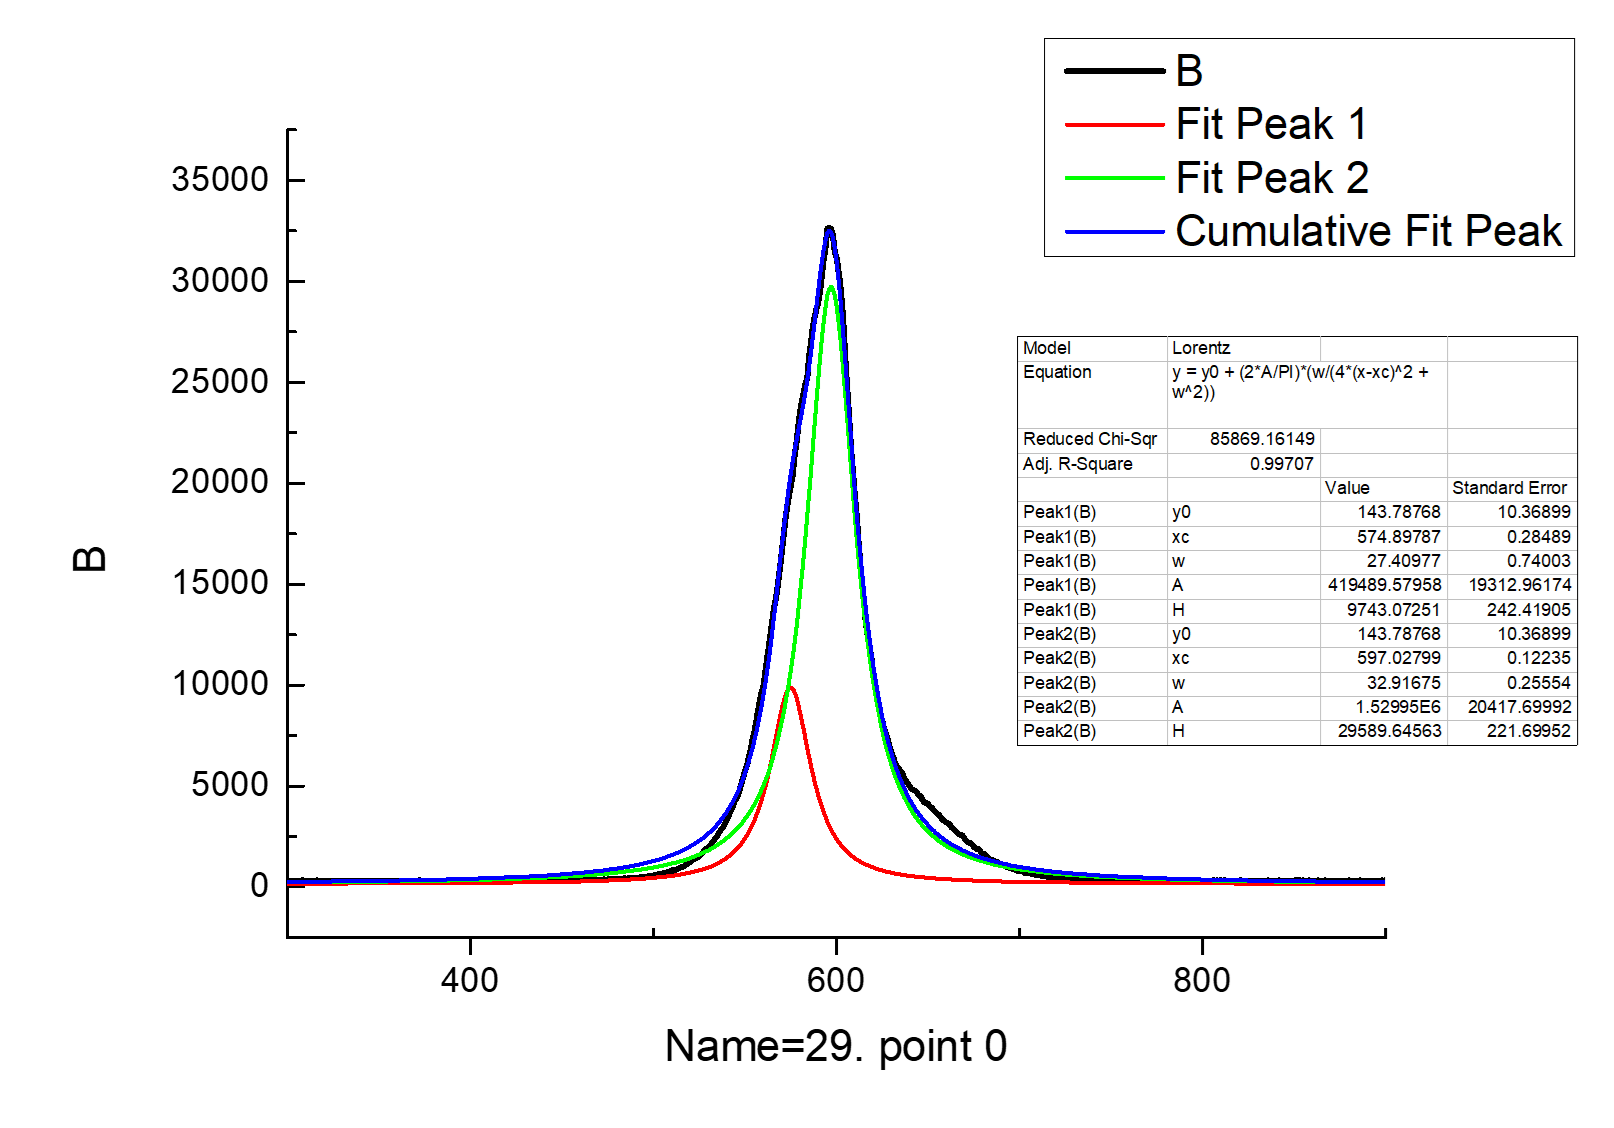
\includegraphics[width=0.8\textwidth]{point0}
		\end{tabular}
	\end{center}
	\caption{The PL data of the set point 0 is shown by sum of exciton and biexciton peak.}
	\label{fig:point0}  
\end{figure}

Figure \ref{fig:point0}\과 같이 multiple peak fitting을 마친 후에는 각 peak의 x값, 즉 wavelength 값과 y값, 즉 intensity 값을 데이터로 기록한 후 분석하였다.

\subsubsection{Line data analysis}
위의 과정에서 각 point 들의 data에 대한 peak fitting을 한 이후에 그 경향성을 보기 위해 필요한 과정이다. 분석하고자 하는 것은 중앙에서 바깥으로 가면서 peak intensity의 경향성이다. 이를 위해서 peak fitting 과정에서 얻은 데이터인 각 point에서의 biexciton, exciton peak의 intensity값을 y축, point 번호를 x 축으로 설정하여  line 1, line 2, line 3 별로 막대그래프를 그려서 경향성을 볼 수 있었다.
\\

\subsection{분석 결과 및 해석}
Line 1, Line 2, Line 3 에서의 결과를 각각 Figure \ref{fig:line1}, Figure \ref{fig:line2}, Figure \ref{fig:line3}에 나타내었다.

\begin{figure}[H]
	\begin{tabular}{cc}
		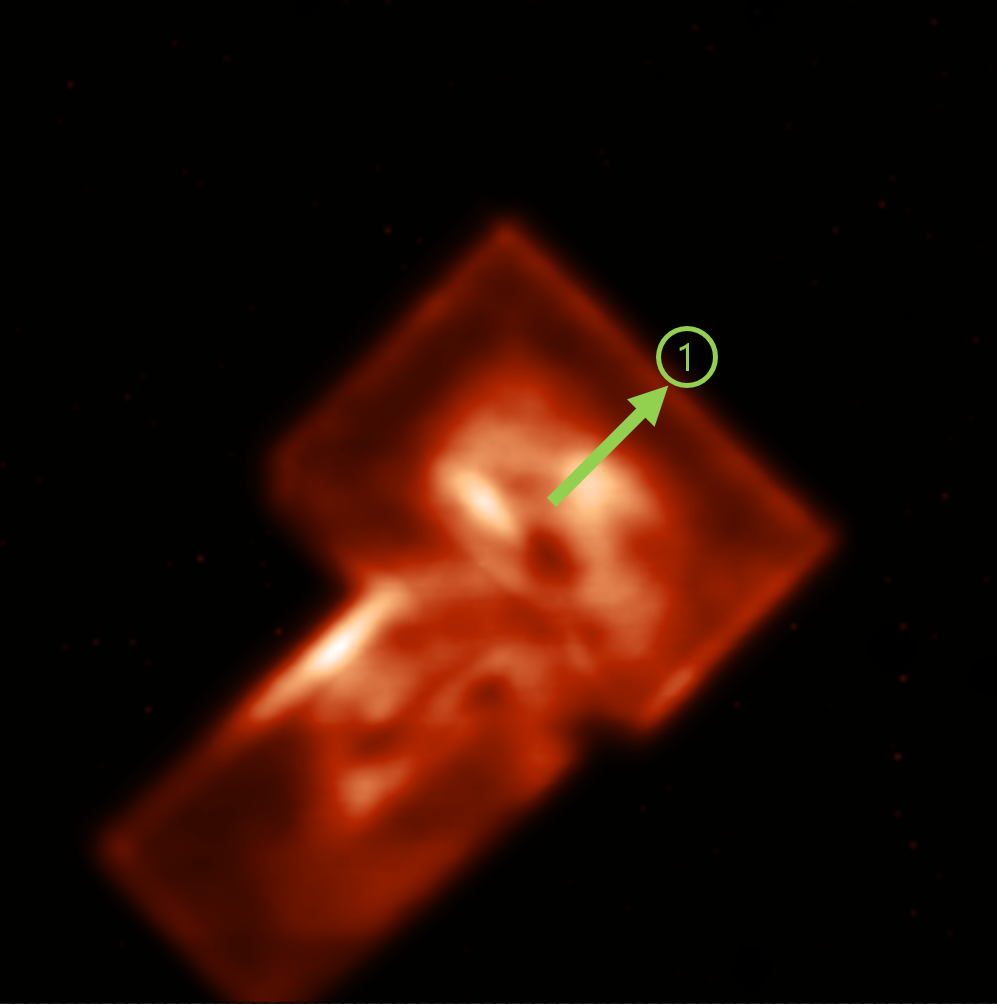
\includegraphics[width=0.3\textwidth]{line1}
		\begin{tikzpicture} [remember picture,overlay]	
		\node[text=white] at (-4, 4) {(a)};
		\end{tikzpicture}
		&
		\begin{tikzpicture}
		\begin{axis} [
		width=0.70\textwidth,%
		height = 5cm,%
		ybar,%
		bar width=5pt,
		title={Line 1},%
		xtick = data,%
		symbolic x coords={0, 1, 2, 3, 4, 5, 6, 7, 8},%
		xlabel= {Viewpoint},%
		ylabel= {Intensity(a.u.)},%
		ymin=0,ystep=5000,ymax=35000.0,%
		scaled y ticks = false,%
		ymajorgrids = true,
		legend style={at={(0.02,10)}},legend pos=north east]%
		\addplot table [x=no, y=biexciton] {./data/line1.csv}; %
		\addlegendentry {biexciton}%
		\addplot table [x=no, y=exciton] {./data/line1.csv}; %
		\addlegendentry {exciton}%
		\end{axis}
		\node at (-0.9, 3.5) {(b)};
		\end{tikzpicture}
	\end{tabular}
	\caption{(a) Route set to line 1, (b) Analyzed data :tendency in the path along line 1.}
	\label{fig:line1}  
\end{figure}




Figure \ref{fig:line1}, 즉 line 1에서는 exciton과 biexciton 모두 감소하는 추세를 보이다가 끝에서 증가하는 모습을 볼 수 있다.

\begin{figure}[H]
	\begin{tabular}{cc}
		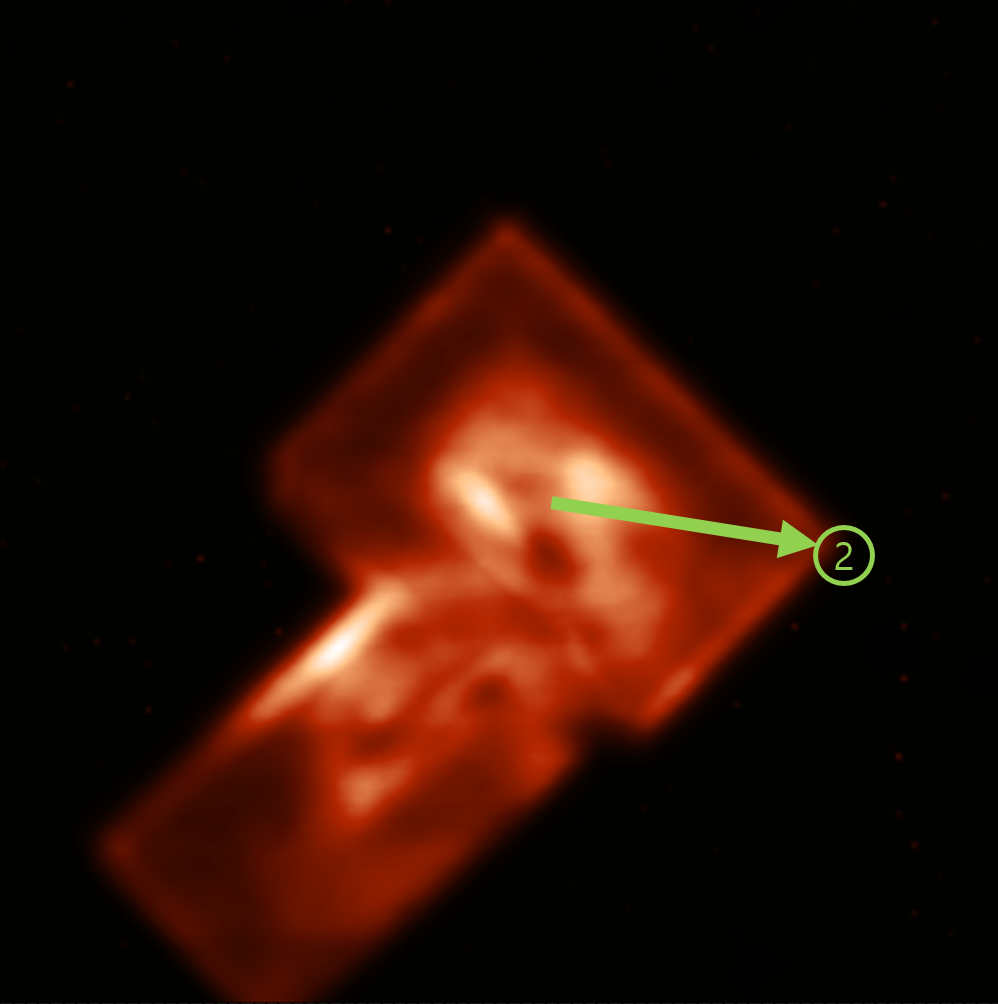
\includegraphics[width=0.3\textwidth]{line2}
		\begin{tikzpicture} [remember picture,overlay]	
		\node[text=white] at (-4, 4) {(a)};
		\end{tikzpicture}
		&
		\begin{tikzpicture}
		\begin{axis} [
		width=0.70\textwidth,%
		height = 5cm,%
		ybar,%
		bar width=5pt,
		title={Line 2},%
		xtick = data,%
		symbolic x coords={0, 1, 2, 3, 4, 5, 6, 7, 8, 9, 10, 11},%
		xlabel= {Viewpoint},%
		ylabel= {Intensity(a.u.)},%
		ymin=0,ystep=5000,ymax=35000.0,%
		scaled y ticks = false,%
		ymajorgrids = true,
		legend style={at={(0.02,10)}},legend pos=north east]%
		\addplot table [x=no, y=biexciton] {./data/line2.csv}; %
		\addlegendentry {biexciton}%
		\addplot table [x=no, y=exciton] {./data/line2.csv}; %
		\addlegendentry {exciton}%
		\end{axis}
		\node at (-0.9, 3.5) {(b)};
		\end{tikzpicture}
	\end{tabular}
	\caption{(a) shows the route set to line 2. (b)  is the analyzed data and shows the tendency in the path along line 2.}
	\label{fig:line2}  
\end{figure}


Figure \ref{fig:line2}, 즉 line 2에서는 exciton과 biexciton 모두 감소하는 추세를 보이다가 가장 끝 두점에서는 biexciton은 급격히 증가, exciton은 급격히 감소함을 볼 수 있다.

\begin{figure}[H]
	\begin{tabular}{cc}
		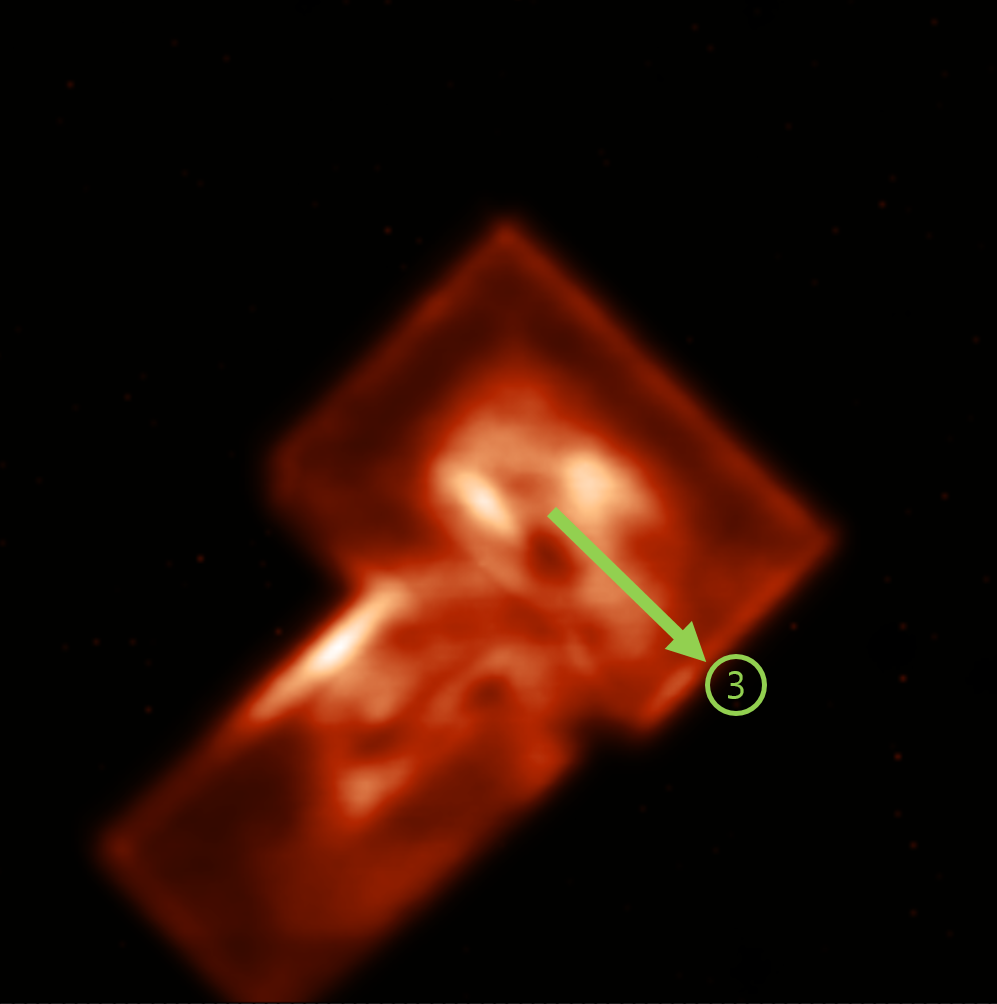
\includegraphics[width=0.3\textwidth]{line3}
		\begin{tikzpicture} [remember picture,overlay]	
		\node[text=white] at (-4, 4) {(a)};
		\end{tikzpicture}
		&
		\begin{tikzpicture}
		\begin{axis} [
		width=0.70\textwidth,%
		height = 5cm,%
		ybar,%
		bar width=5pt,
		title={Line 3},%
		xtick = data,%
		symbolic x coords={0, 1, 2, 3, 4, 5, 6, 7, 8, 9, 10, 11, 12, 13, 14},%
		xlabel= {Viewpoint},%
		ylabel= {Intensity(a.u.)},%
		ymin=0,ystep=5000,ymax=35000.0,%
		scaled y ticks = false,%
		ymajorgrids = true,
		legend style={at={(0.02,10)}},legend pos=north east]%
		\addplot table [x=no, y=biexciton] {./data/line3.csv}; %
		\addlegendentry {biexciton}%
		\addplot table [x=no, y=exciton] {./data/line3.csv}; %
		\addlegendentry {exciton}%
		\end{axis}
		\node at (-0.9, 3.5) {(b)};
		\end{tikzpicture}
	\end{tabular}
	\caption{(a) shows the route set to line 3. (b)  is the analyzed data and shows the tendency in the path along line 3.}
	\label{fig:line3}  
\end{figure}





Figure \ref{fig:line3}, 즉 line 3에서는 exciton은 감소, biexciton은 증가하는 추세를 보이다가 가장 끝 두 점에서는 biexciton은 급격히 감소, exciton은 급격히 증가함을 볼 수 있다.

세 line에서 exciton, biexciton 각각의 공통되는 경향성이나 규칙은 찾아보기 어렵다. 하지만 중앙에서 중간까지 갈 때는 특정한 경향성을 보이는 듯하다가 가장 바깥, 가장자리에서 그 경향성이 반대되는 모습을 볼 수 있다. 종합적으로 보았을 때는 가장자리로 가면서 감소하는 모습을 보이다가 다시 증가하는 모습이 세 line 모두에서 나타났다.

같은 ND2로 찍은 PL 데이터를 관찰했을 때, 완전한 가장자리를 제외하면 바깥으로 갈수록 biexciton peak의 상대적인 세기가 세짐을 관찰할 수 있었다. 

PL 측정 시 $\rm CsPbBr_3$가 구조상의 deformation이 일어나지 않으므로 비슷한 양의 carrier가 전도띠로 가는 것은 자명하다. 이 carrier들은 각각 exciton이나 biexciton의 형태로 존재하게 되는데, PL에서 biexciton에 의한 peak가 더 우세하게 관찰된 것이라고 해석할 수 있다.


		
	\section{Results}


\subsection{Outflow Identification}

\begin{table}[h!]
	\caption{Protostars with observed outflows.}
	\label{table:protostars}
	\begin{center}
		\begin{tabular}{c|c|c|c|c}
			\toprule
			& \multicolumn{2}{c|}{Coordinates} & $\mathbf{L_{bol}}$ & $\mathbf{T_{bol}}$\\
			\textbf{Name} & \textbf{RA} & \textbf{Dec} & $\mathbf{[L_{\odot}]}$ & $\mathbf{[K]}$\\
			\midrule
			\centering
			FIR2 & 05:35:24.3 & -05:08:33.3 & 5.68 & 100.6\\
			FIR3 & 05:35:27.5 & -05:09:32.5 & 360.86 & 71.5\\
			FIR6b & 05:35:23.4 & -05:12:03.2 & 21.93 & 54.1\\
			MMS2 & 05:35:18.3 & -05:00:34.8 & 20.11 & 186.3\\
			MMS5 & 05:35:22.4 & -05:01:14.1 & 15.81 & 42.4\\
			MMS9 & 05:35:26.0 & -05:05:42.4 & 8.91 & 38.1\\
			\midrule
		\end{tabular}
	\end{center}
\end{table}

Table \ref{table:protostars} shows the protostars with bipolar outflows observed. The names of the protostars are from the $1.3\textrm{mm}$ continuum observations by Chini et al. \cite{chini1997dust} and Nielbock et al. \cite{nielbock2003stellar} $L_{bol}$ and $T_{bol}$ were calculated from the Spitzer and Herschel surveys \cite{megeath2012spitzer, furlan2016herschel}.

\newpage
\subsubsection{$^{12}$CO J = 2 - 1 Observations}

\begin{figure}[h!]
	\begin{center}
		\begin{tabular}{cc}
			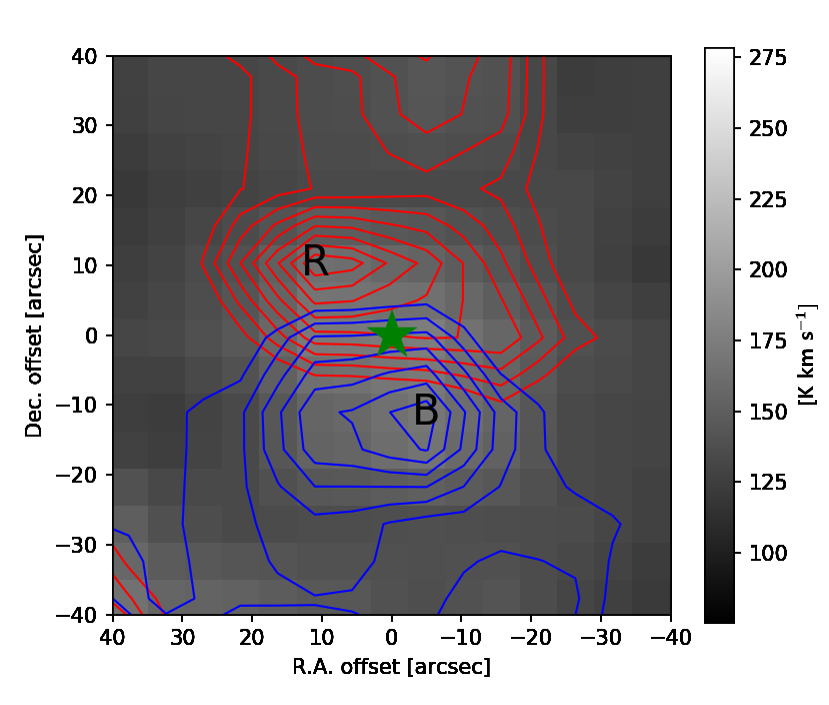
\includegraphics[width=7cm]{Orion_12CO2-1_FIR2_rbcontour_400_modified} &   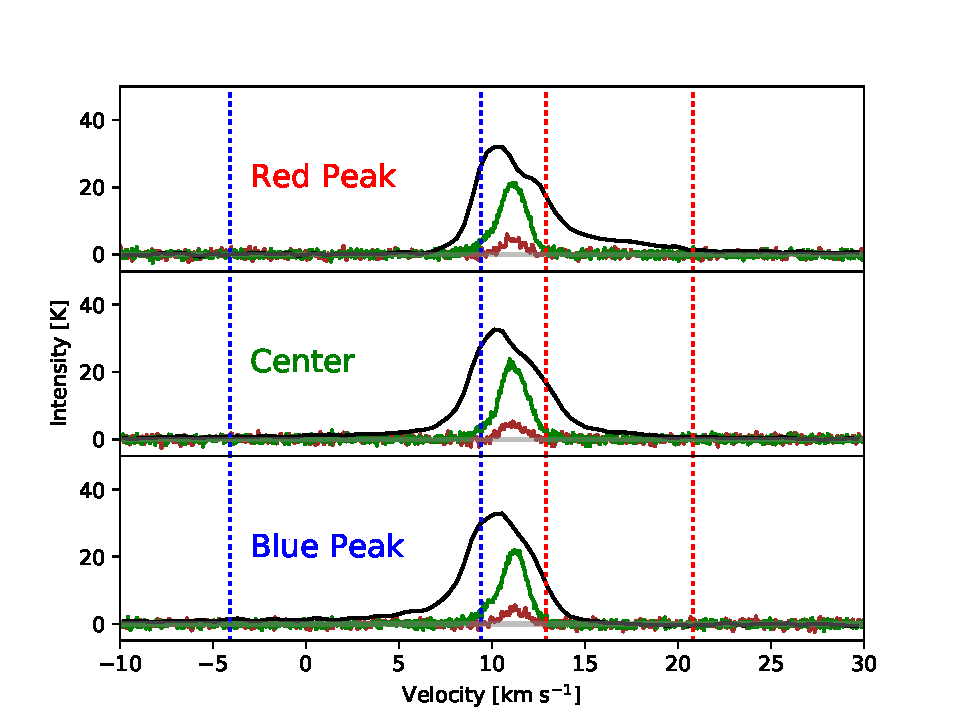
\includegraphics[width=7cm]{Orion_12CO2-1_FIR2_line_profile_400}
		\end{tabular}
		\caption{The $^{12}$CO J = 2 - 1 intensity contour map (left) and the line profile (right) of FIR2.}	
	\label{fig:FIR221}
	\end{center}
\end{figure}

\begin{figure}[h!]
	\begin{center}
		\begin{tabular}{cc}
			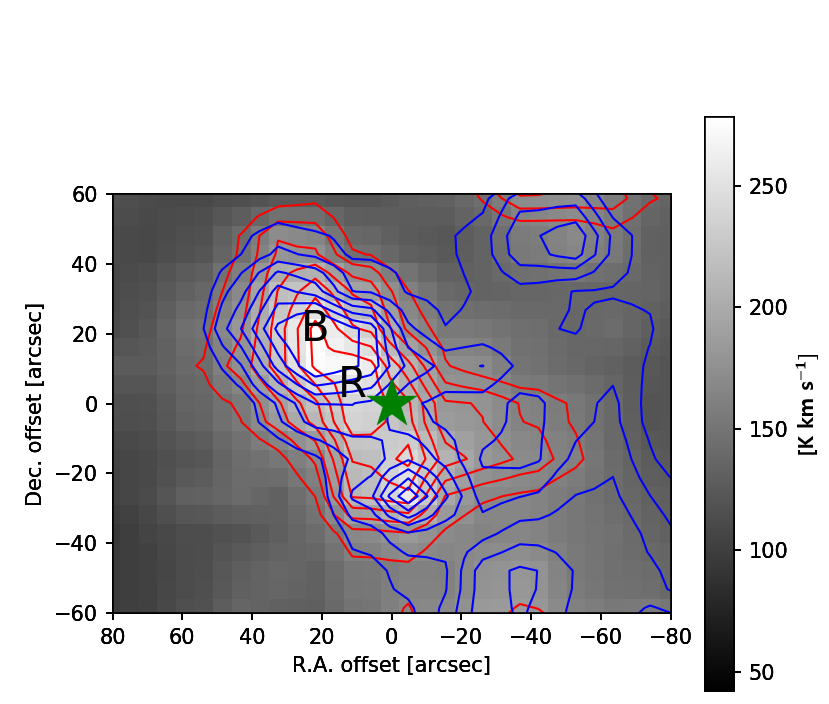
\includegraphics[width=7cm]{Orion_12CO2-1_FIR3_rbcontour_400_modified} &   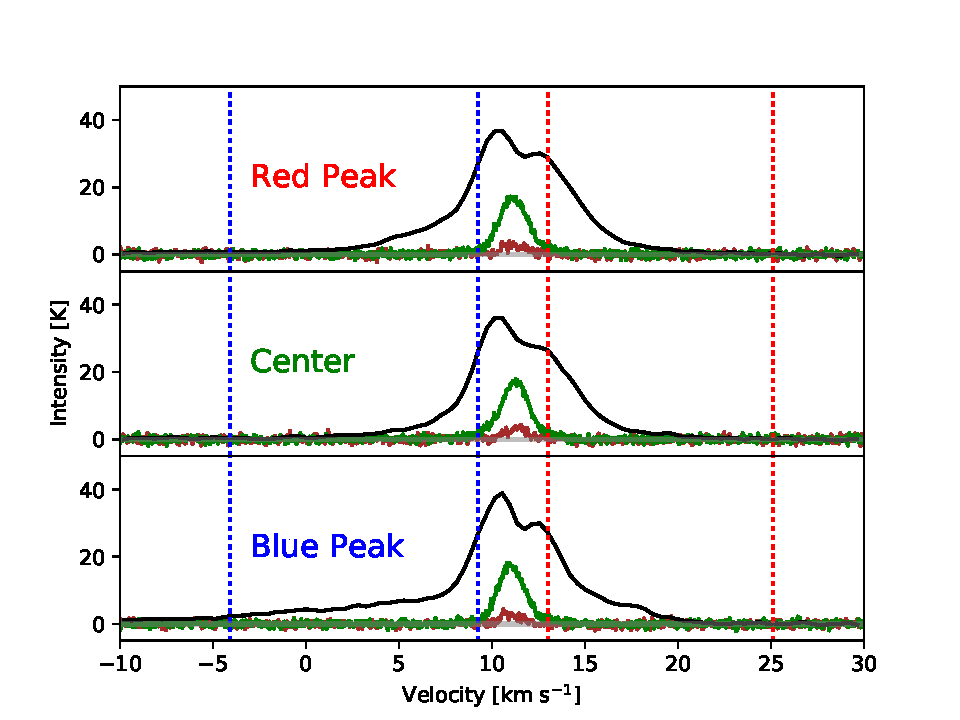
\includegraphics[width=7cm]{Orion_12CO2-1_FIR3_line_profile_400}
		\end{tabular}
		\caption{The contour map and the line profile of FIR3.}
	\label{fig:FIR321}
	\end{center}
\end{figure}

\begin{figure}[h!]
	\begin{center}
		\begin{tabular}{cc}
			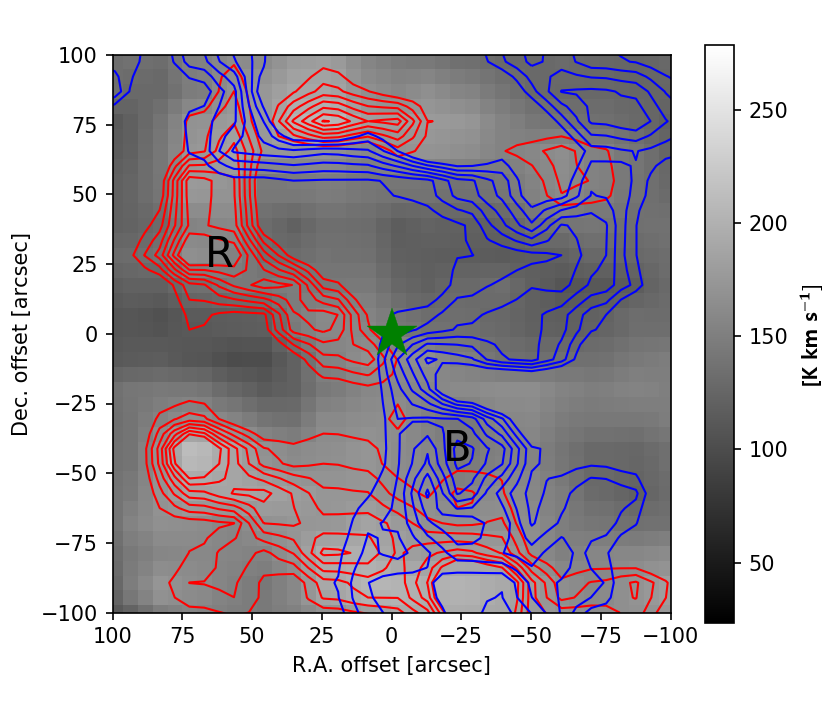
\includegraphics[width=7cm]{Orion_12CO2-1_FIR6b_rbcontour_400_modified} &   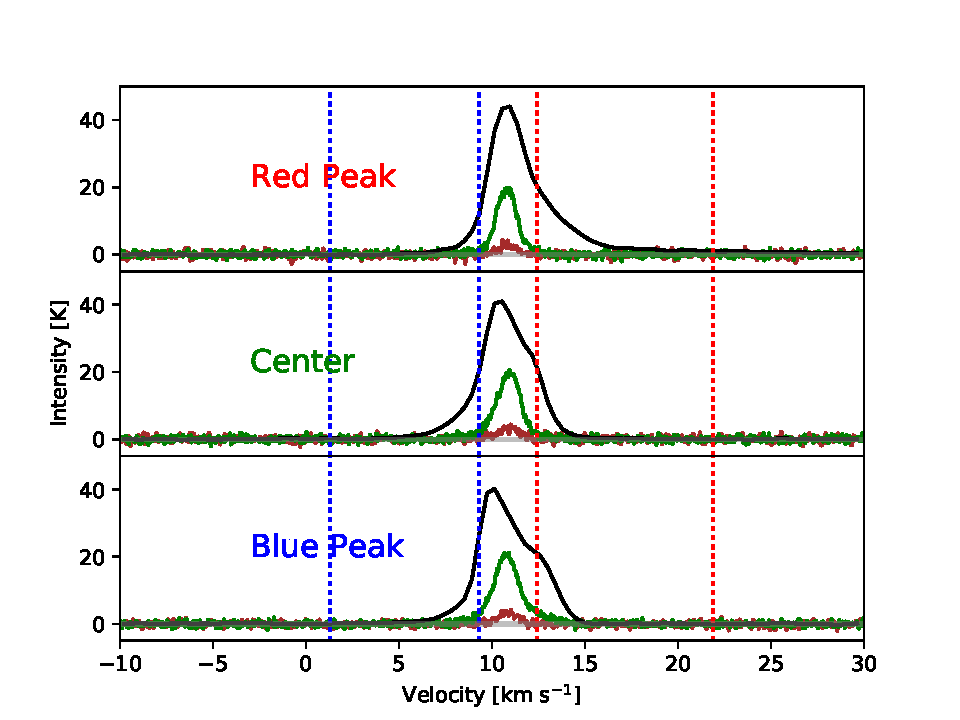
\includegraphics[width=7cm]{Orion_12CO2-1_FIR6b_line_profile_400}
		\end{tabular}
		\caption{The contour map and the line profile of FIR6b. }
	\label{fig:FIR6b21}
	\end{center}
\end{figure}

\begin{figure}[h!]
	\begin{center}
		\begin{tabular}{cc}
			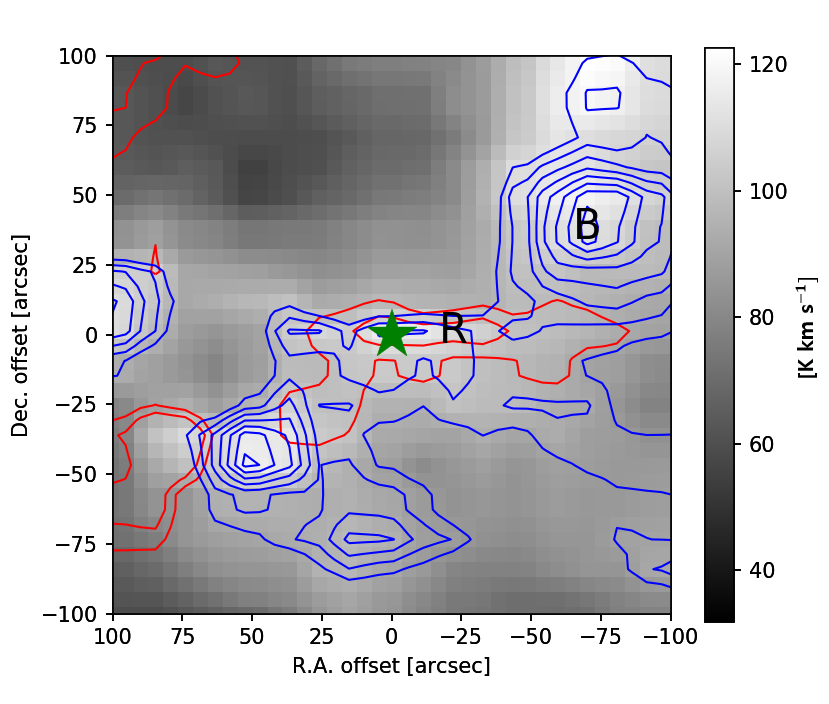
\includegraphics[width=7cm]{Orion_12CO2-1_MMS2_rbcontour_400_modified} &   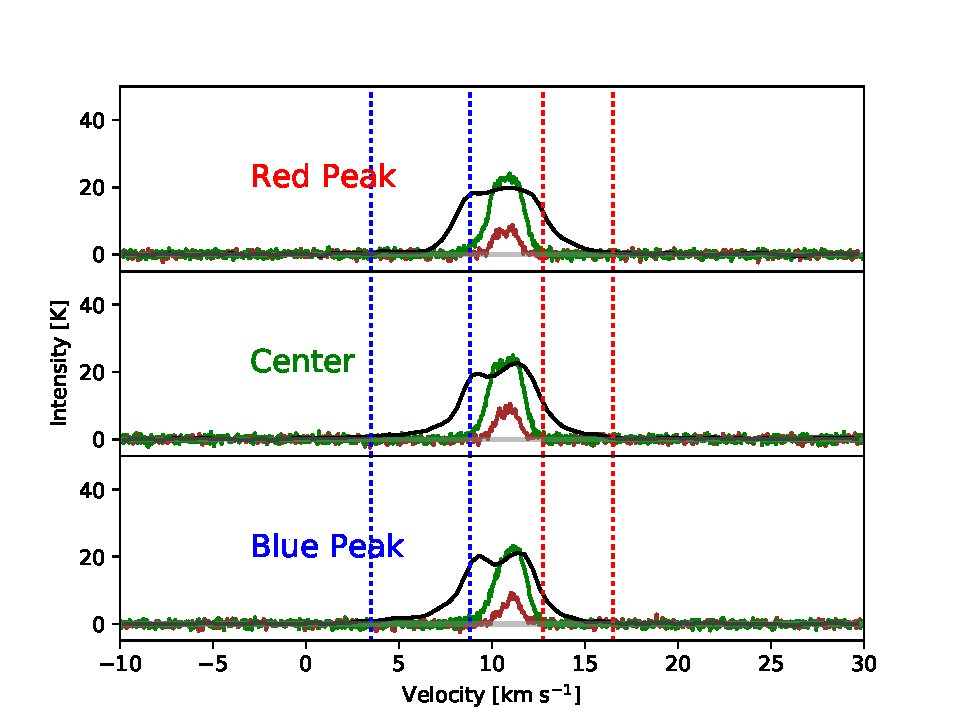
\includegraphics[width=7cm]{Orion_12CO2-1_MMS2_line_profile_400}
		\end{tabular}
		\caption{The contour map and the line profile of MMS2. }
	\label{fig:MMS221}
	\end{center}
\end{figure}

\begin{figure}[h!]
	\begin{center}
		\begin{tabular}{cc}
			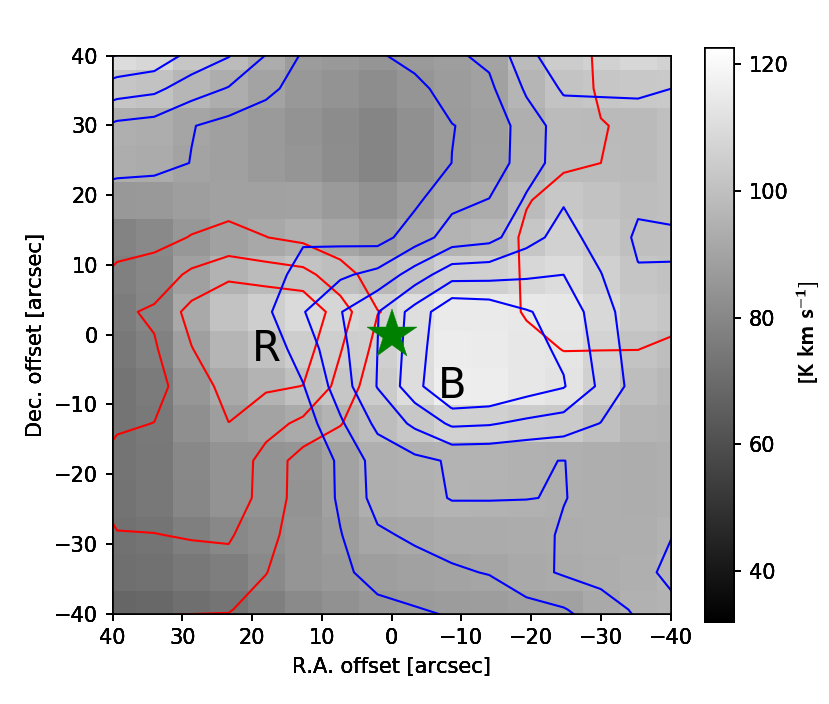
\includegraphics[width=7cm]{Orion_12CO2-1_MMS5_rbcontour_400_modified} &   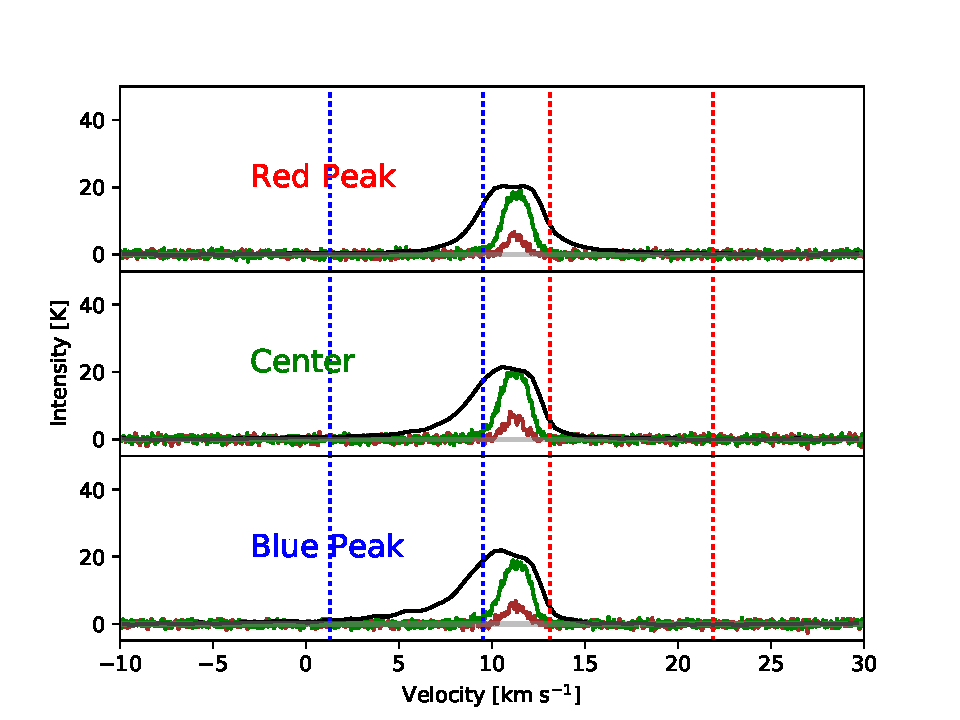
\includegraphics[width=7cm]{Orion_12CO2-1_MMS5_line_profile_400}
		\end{tabular}
		\caption{The contour map and the line profile of MMS5. }
	\label{fig:MMS521}
	\end{center}
\end{figure}

\begin{figure}[h!]
	\begin{center}
		\begin{tabular}{cc}
			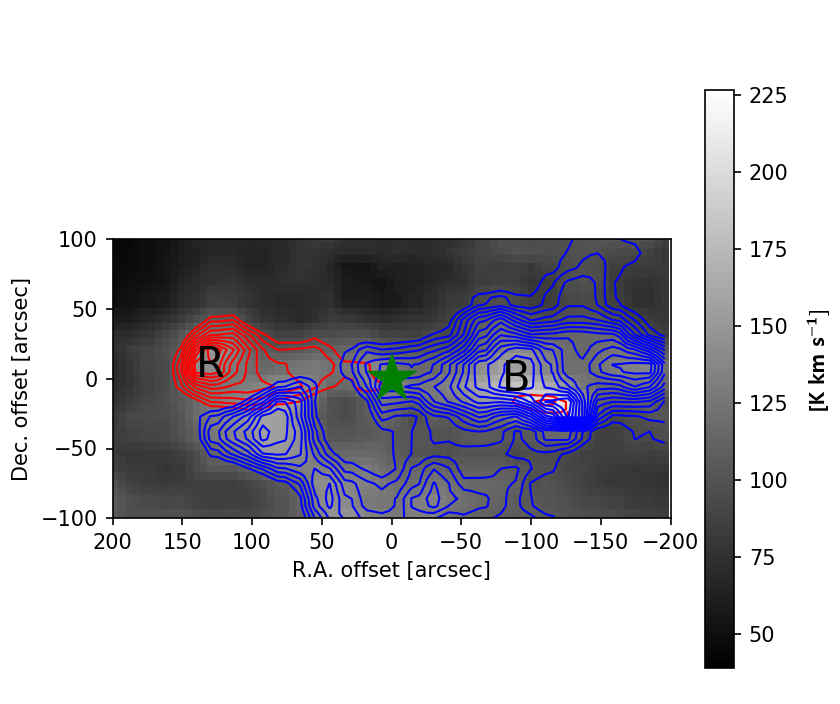
\includegraphics[width=7cm]{Orion_12CO2-1_MMS9_rbcontour_400_modified} &   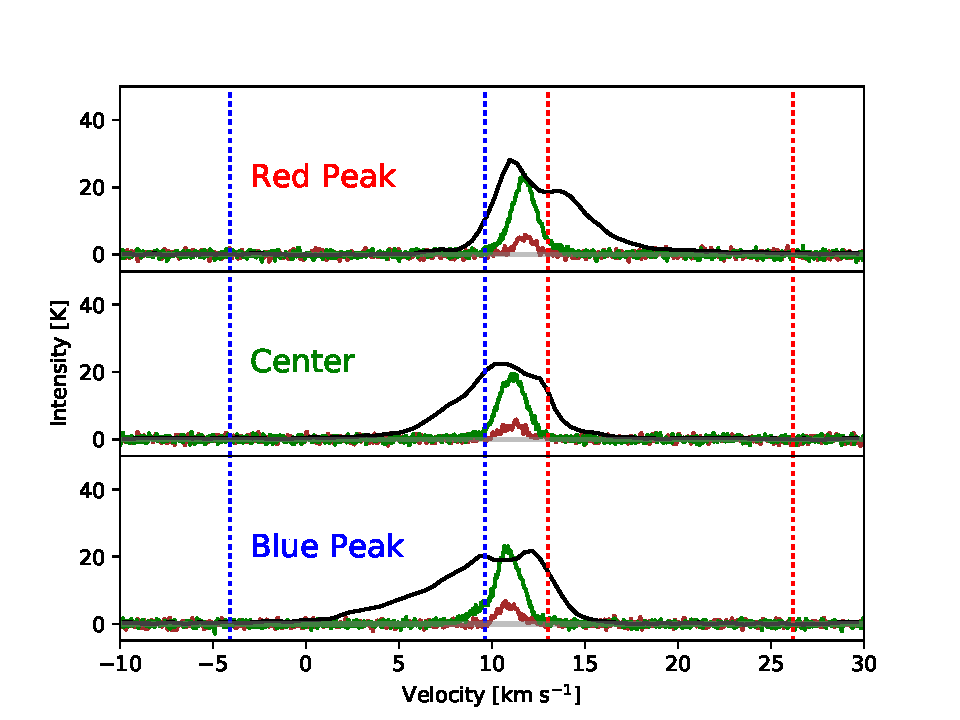
\includegraphics[width=7cm]{Orion_12CO2-1_MMS9_line_profile_400}
		\end{tabular}	
		\caption{The contour map and the line profile of MMS9. }
	\label{fig:MMS921}
	\end{center}
\end{figure}

\clearpage
\newpage
\noindent The $^{12}$CO J = 2 - 1 intensity for each point were calculated by using equations (\ref{column_density}) and (\ref{beam_mass}). The line profile shows the intensities of $^{12}$CO J = 2 - 1 (black), $^{13}$CO J = 1 - 0 (green), and C$^{18}$O J = 1 - 0 (brown) for each point. 

\noindent\textit{FIR2} -- There is a strong bipolar outflow elongated along the N-S direction as shown in Figure \ref{fig:FIR221}. The size is about 30 arcsec, which is smaller than other outflows detected. Red and blue contour intervals are $10\sigma$ starting from $60\sigma$ and $10\sigma$ starting from $100\sigma$ respectively.\\
\textit{FIR3} -- A strong bipolar outflow can be seen along NE-SW direction, with red and blue lobes overlapping each other as shown in Figure \ref{fig:FIR321}. This tells us that the outflow axis is almost parallel to the line of sight. Red and blue contour intervals are $20\sigma$ starting from $40\sigma$ and $20\sigma$ starting from $60\sigma$ respectively. \\
\textit{FIR6b} -- The contour is not so clear because of other IR sources nearby as shown in Figure \ref{fig:FIR6b21}. The outflow is along the NW-SE direction. Red and blue contour intervals are $10\sigma$ starting from $45\sigma$ and $10\sigma$ starting from $110\sigma$ respectively.\\
\textit{MMS2} -- The contour is in a tricky situation, because both red and blue lobes are on the east side of the protostar as shown in Figure \ref{fig:MMS221}. The outflow structure on the SW side is the outflow from another protostar, MMS5. It is possible that the outflow structure changed shape because of the turbulence from other protostars. Red and blue contour intervals are $10\sigma$ starting from $30\sigma$ and $10\sigma$ starting from $60\sigma$ respectively.\\
\textit{MMS5} -- There is an outflow structure along the E-W direction as shown in Figure \ref{fig:MMS521}. This outflow is much smaller than other bipolar outflows. Red and blue contour intervals are $10\sigma$ starting from $20\sigma$ and $10\sigma$ starting from $40\sigma$ respectively.\\
\textit{MMS9} -- There is a strong outflow along the E-W direction as shown in Figure \ref{fig:MMS921}. We can see a smaller red lobe near the center of the blue lobe. Red and blue contour intervals are $10\sigma$ starting from $50\sigma$ and $10\sigma$ starting from $60\sigma$ respectively.\\

\subsubsection{$^{12}$CO J = 1 - 0 Observations}

%%%박기현 수정 시작
\begin{figure}[h!]
	\begin{tabular}{ccc}
		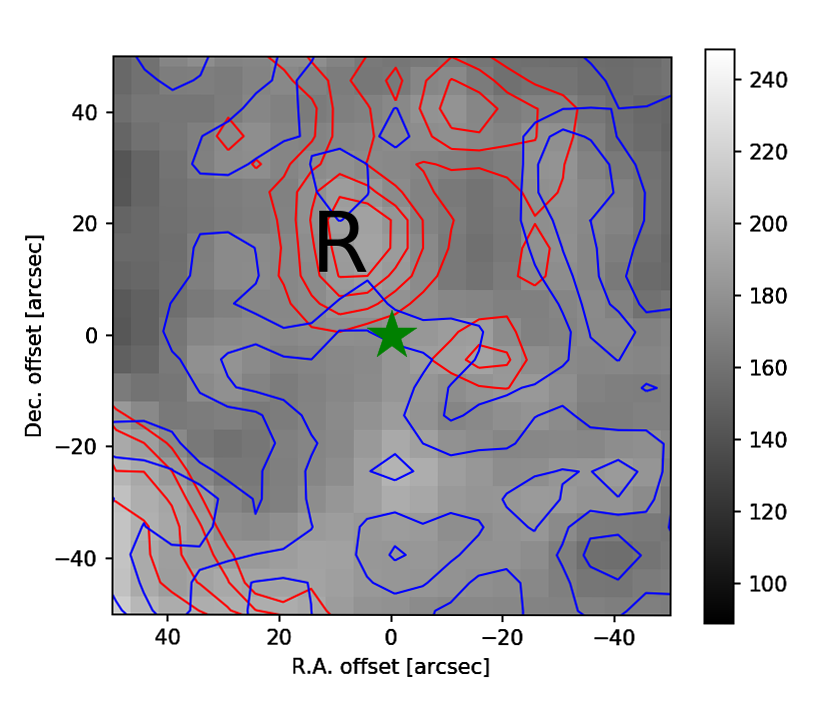
\includegraphics[width = 4.3cm]{Orion_12CO_NRO_HOPS68_rbcontour_400} & 
		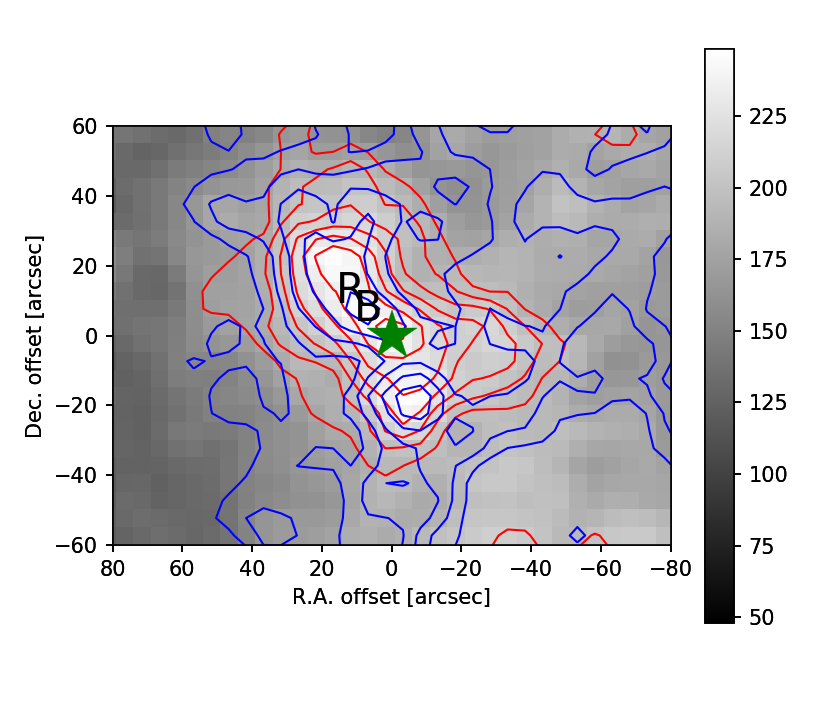
\includegraphics[width = 4.6cm]{Orion_12CO_NRO_HOPS370_rbcontour_400} & 
		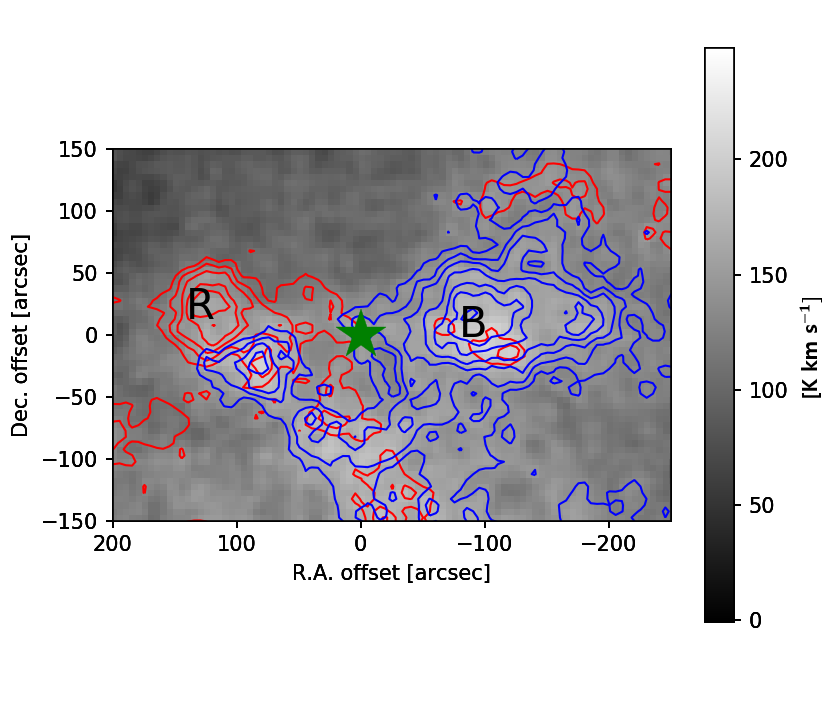
\includegraphics[width = 4.6cm]{Orion_12CO_NRO_HOPS78_rbcontour_400}		
	\end{tabular}
	\caption{The $^{12}$CO J = 1 - 0 intensity contour map of FIR2 (left), FIR3 (middle), and MMS9 (right). }
	\label{fig:12COcontourmap}
\end{figure}
%%%박기현 수정 끝

%%%선재 원본
%%%\begin{figure}[h!]
%%%	\begin{tabular}{ccc}
%%%		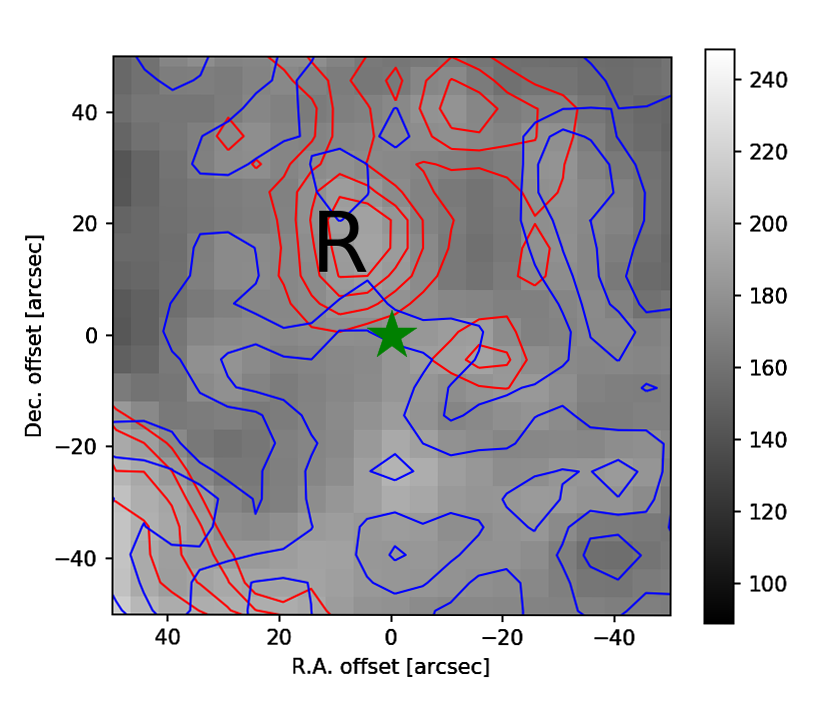
\includegraphics[width = 5cm]{Orion_12CO_NRO_HOPS68_rbcontour_400.png} & 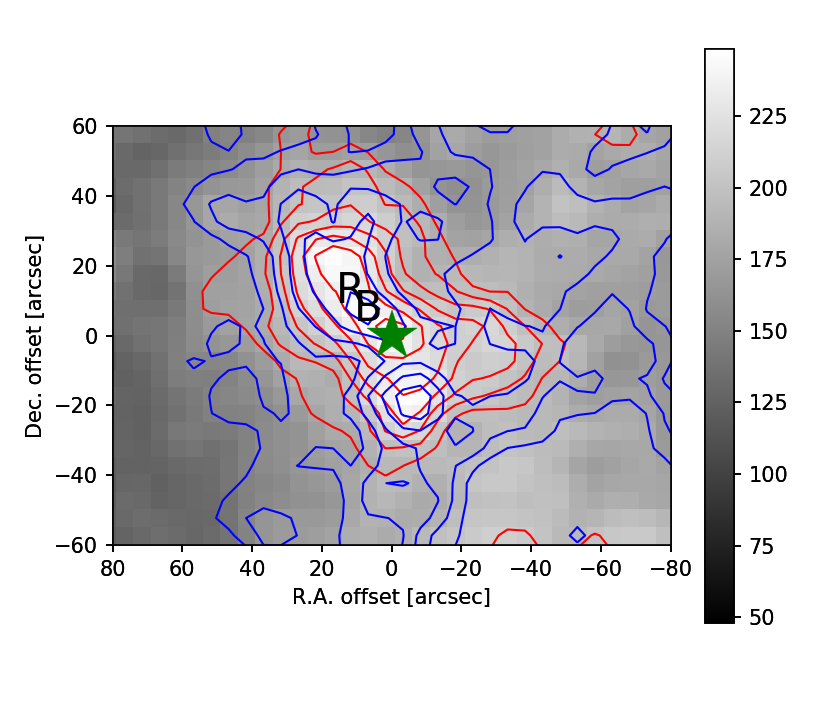
\includegraphics[width = 5cm]{Orion_12CO_NRO_HOPS370_rbcontour_400.png} & 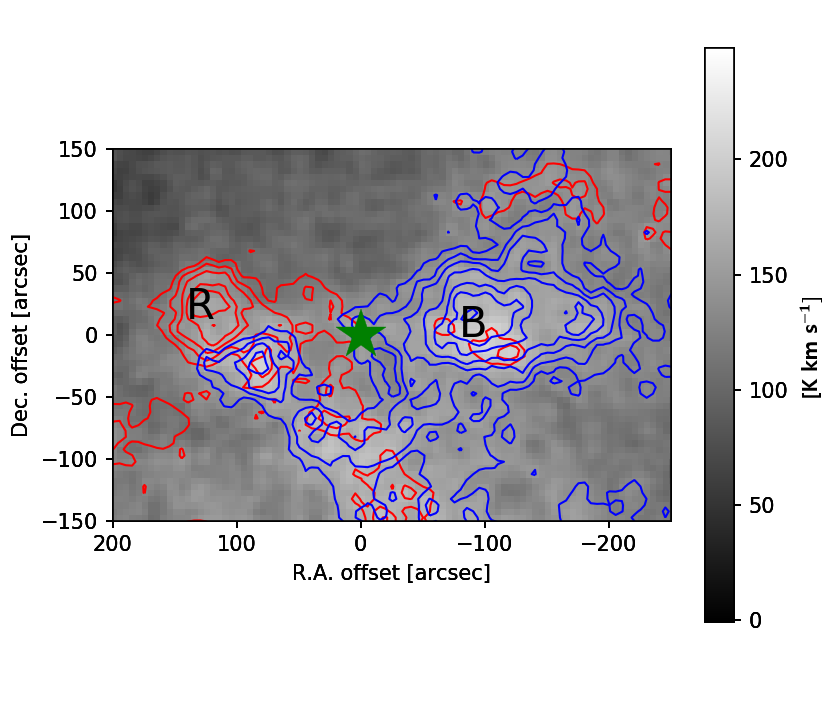
\includegraphics[width = 5cm]{Orion_12CO_NRO_HOPS78_rbcontour_400.png}
%%%		\label{10}
%%%	\end{tabular}
%%%	\caption{The contour map of FIR2(left), FIR3(middle), and MMS9(right). }
%%%\end{figure}
%%%선재 원본
 
\noindent \textit{FIR2} -- The red lobe is clear on the NW side of the protostar, but the blue lobe is not as clear as shown in Figure \ref{fig:12COcontourmap}.\\
\textit{FIR3} -- The outflows are in a similar shape as the J = 2 - 1 observations as shown in Figure \ref{fig:12COcontourmap}. The lobe centers are slightly near the protostar.\\
\textit{MMS9} -- The outflows are also in a similar shape as the J = 2 - 1 observations as shown in Figure \ref{fig:12COcontourmap}. We can also see that there is a small red lobe near the center of the blue lobe.\\
\newpage

\subsection{Momentum Flux}


\begin{table}[h]
	\caption{CO outflow parameters.} \label{table:result}
	\begin{center}
		\begin{tabular}{c|c|c|c||c|c|c}
			\toprule
			\multirow{3}{1cm}{\textbf{Name}} & \multicolumn{3}{c}{J = 2 - 1} & \multicolumn{3}{c}{J = 1 - 0} \\
			& $\mathbf{F_{R}}$ & $\mathbf{F_{B}}$ & $\mathbf{F_{\textrm{\textbf{CO}}}}$ & $\mathbf{F_{R}}$ & $\mathbf{F_{B}}$ & $\mathbf{F_{\textrm{\textbf{CO}}}}$\\
			& \multicolumn{6}{c}{($M_{\odot} \, \textrm{km s}^{-1} \textrm{yr}^{-1}$)}\\
			\midrule
			FIR2 & 1.14E-05 & 3.28E-05 & 4.42E-05 & 4.78E-06 & - & 4.78E-06\\
			FIR3 & 4.77E-04 & 7.43E-04 & 1.22E-03 & 1.86E-04 & 3.02E-04 & 4.88E-04\\
			FIR6b & 1.13E-05 & 1.18E-05 & 2.31E-05 & - & - & -\\
			MMS2 & 1.14E-05 & 4.50E-05 & 5.64E-05 & - & - & -\\
			MMS5 & 5.80E-06 & 1.55E-05 & 2.13E-05 & - & - & -\\
			MMS9 & 3.67E-06 & 1.09E-05 & 1.46E-05 & 1.45E-06 & 6.02E-06 & 7.47E-06\\
			\toprule
		\end{tabular}
	\end{center}
\end{table}


\noindent Table \ref{table:result} shows the parameters of the outflows detected. $F_R$ and $F_B$ stands for the outflow forces for the red lobe and the blue lobe respectively. $F_{CO}$ is calculated by adding the two forces, which shows the momentum flux of the protostar. We can see that more outflows were detected by using J = 2 - 1 data, and the momentum flux is 2-3 times higher.\\

\clearpage
\newpage
\subsection{Momentum flux vs. Bolometric luminosity}

\begin{figure}[b!]
	\centering
	\includegraphics[width=0.95\textwidth]{Luminosity}
	\caption{CO outflow momentum flux vs. $L_{bol}$}
	\label{fig:lum}
\end{figure}

Figure \ref{fig:lum} shows the relation between the bolometric luminosity and the momentum flux of the outflows from previous studies and this work \cite{takahashi2008millimeter, van2013outflow, hogerheijde1998envelope, nakamura2012evidence, aso2000dense, zhang2005search}.
Since the momentum flux of the same protostar is known to vary somewhat depending on the calculation methods\cite{van2013outflow}, the relation between the bolometric luminosity and the momentum flux is difficult to express with an exact formula and only the degree of tendency can be analyzed.

Orion A Cloud is a region where stars with medium mass are formed. The fact that the momentum flux of the outflow is proportional to the bolometric luminosity can be confirmed.	


%%%
%%%Figure \ref{fig:lum} shows the relation between the bolometric luminosity and the momentum flux of the outflows from previous studies \cite{takahashi2008millimeter, van2013outflow, hogerheijde1998envelope, nakamura2012evidence, aso2000dense, zhang2005search}. \\ Since the momentum flux of the same protostar is known to vary somewhat depending on the calculation methods\cite{van2013outflow}, the relation between the bolometric luminosity and the momentum flux is difficult to express with the excat formula and only the degree of tendency can be analyzed.
%%%The bolometric luminosity was observed by the Spitzer and Herschel telescopes. Orion A Cloud is a region where stars with medium mass are formed. The fact that the momentum flux of the outflow is proportional to the bolometric luminosity could be checked.


\newpage

\subsection{Momentum flux by emission line energy level}

\begin{figure}[b!]
	\centering
	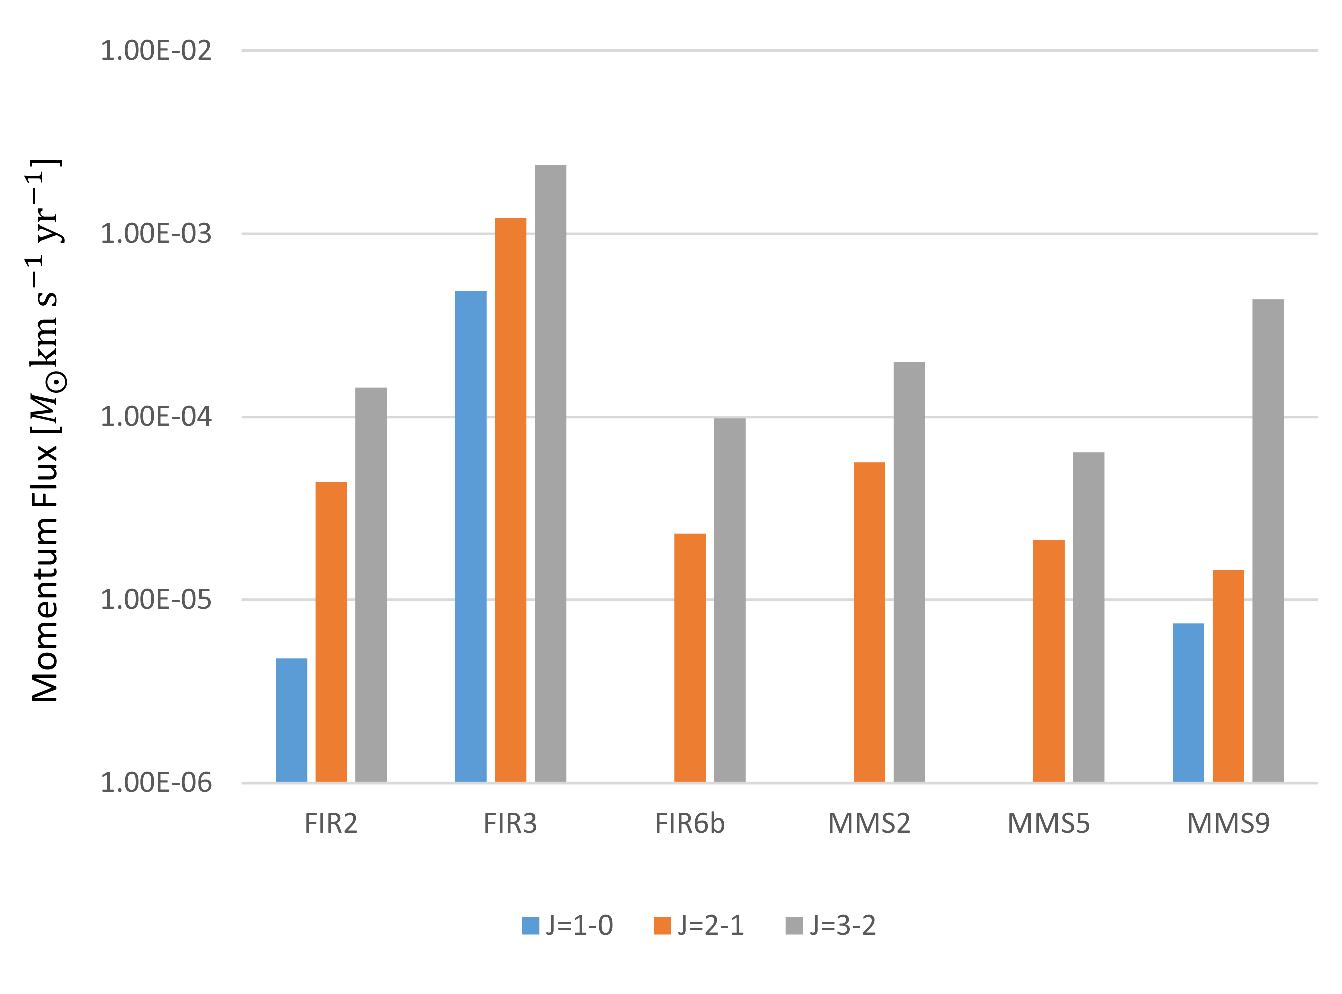
\includegraphics[width=0.9\textwidth]{outflow_J}
	\caption{Momentum flux difference by emission line energy.}
	\label{fig:J}
\end{figure}

Figure \ref{fig:J} compares momentum flux calculated by three different emission lines of the same protostar. The $^{12}$CO J = 3 - 2 observation was made by Takahashi et al \cite{takahashi2008millimeter}. We can see that it is possible to detect more outflows by using a higher energy emission line of $^{12}$CO. Using data with smaller beamwidth also enhances detecting outflows.
 
The reason that higher energy lines can detect more outflows can be explained as the following: The excitation temperature is higher for emission lines with higher energy. Outflows drag out matter from the protostar's envelope, which has higher temperature than its surroundings. Lines with higher energy are emitted, which has an effect that makes column density higher than usual.
	%-----------------------------------------------------
% Conclusion
%-----------------------------------------------------
\newpage

\section{결론	}
본 연구의 주요 결론은 다음과 같다:
\begin{enumerate}
	\item Perovskite $\rm CsPbBr_3$의 single crystal은 PL data 의 경향성을 보았을 때 결정의 바깥 쪽에서 wave guiding effect가 발생하고 있다고 해석할 수 있다.
	\item 결정의 가장자리에서 exciton 과 biexciton의 경향성이 반대가 되며, 종합적으로는 중앙에서 가장자리로 가면서 감소했다가 다시 증가하는 추세를 가지고 있다. 이는 결국 defect가 많은 가장자리로 전자가 많이 모이게 됨을 뜻한다.
\end{enumerate}
PL 데이터로 fitting 한 peak의 intensity가 커진다는 것은 exciton과 biexciton이 생성되는 radiative recombination이 많아진다는 것을 의미하고 이는 defect가 줄어 결정의 순도가 높아지는 것으로 해석할 수 있다.

반대로 생각해보면 중심으로 갈수록 증가하는 PL peak는 결정의 가장자리 부분으로 갈수록 결정의 순도가 낮다고 판단될 만큼의 defect가 존재했다는 것을 의미한다. 하지만 실험 결과를 보면 완전한 가장자리에서는 다시 증가하는 것을 볼 수 있는데, 이는 waveguiding effect에 의한 것으로 보인다. 이론적 배경에서도 언급했듯이 waveguiding effect는 빛이 에너지의 이득을 보기 위해서 특정 장소로 모이게 되는 일이 발생하게 되는 것을 말하는데, 결과를 보면 본 논문도 같은 경우로 보인다.

Defect의 에너지 준위는 전도띠와 원자가띠 사이에 존재하므로, 전도띠에 있는 전자는 가까운 defect의 에너지 준위로 내려가기를 선호한다. 실험 결과를 보았을 때 가장자리로 갈수록 defect가 많았으리라 추정할 수 있다. Defect가 많으면 그 에너지 준위로 전자가 많이 이동하기 때문에 이것이 가장자리로 에너지가 모이는 waveguiding effect를 발생시킨다고 볼 수 있다. % Conclusion
	
	%%\clearpage  %%% Appendix를 새 페이지에서 시작
\appendix
\renewcommand{\thesection}{\Alph{section}} %%% TOC에 appendix numbering 재설정
\renewcommand{\thesubsection}{\arabic{subsection}}
\renewcommand{\thesubsubsection}{\arabic{subsubsection}}
\titleformat{\section}[hang] {\normalfont\fontsize{21}{21}\selectfont\bfseries}{\Alph{section}.}{1em}{} %%% Appendix section title의 재설정
\titleformat{\subsection}[hang] {\normalfont\fontsize{16}{16}\selectfont\bfseries}{\Alph{section}.\arabic{subsection}.}{1em}{}
\titleformat{\subsubsection}[hang] {\normalfont\fontsize{14}{14}\selectfont}{\Alph{section}.\arabic{subsection}.\arabic{subsubsection}.}{1em}{}
\titleformat{\paragraph}[hang] {\normalfont\fontsize{12}{12}\selectfont\it}{}{1em}{}
\renewcommand{\theequation}{\thesection.\arabic{equation}} %%% Appendix equation numbering 의 재설정
\renewcommand{\thefigure}{\thesection-\arabic{figure}} %%% Appendix figure numbering 의 재설정
\renewcommand{\thetable}{\thesection-\arabic{table}} %%% Appendix table numbering 의 재설정
\setcounter{equation}{0} %%% Appendix equation starting number의 초기화
\setcounter{figure}{0} %%% Appendix figure starting number의 초기화
\setcounter{table}{0} %%% Appendix table starting number의 초기화
\section{부록}
\begin{table}[h!]
	\begin{center}
		\begin{tabular}{c|c|c|c|c|c|c|c|c}
			\toprule
			&\multicolumn{4}{c|}{Previous Work} & \multicolumn{4}{c}{Our Work}\\
			&\multicolumn{2}{c|}{Blue Lobe} & \multicolumn{2}{c|}{Red Lobe} & \multicolumn{2}{c|}{Blue Lobe} & \multicolumn{2}{c}{Red Lobe}\\
			\textbf{Name} & $\mathbf{v_{out}}$ & $\mathbf{v_{in}}$ & $\mathbf{v_{out}}$ & $\mathbf{v_{in}}$&$\mathbf{v_{out}}$ & $\mathbf{v_{in}}$ & $\mathbf{v_{out}}$ & $\mathbf{v_{in}}$\\
			& [km/s] & [km/s] & [km/s] & [km/s] & [km/s] & [km/s] & [km/s] & [km/s] \\ 
			\midrule
			\multicolumn{9}{c}{Orion A Cloud}\\
			\midrule
			FIR2 & -4.1 & 8.9 & 13.2 & 20.8 &-4.1 & 9.4 & 12.9 & 20.8\\
			FIR3 & -4.1 & 8.9 & 13.2 & 25.1 & -4.1 & 9.25 & 13.0 & 25.1\\
			FIR6b & 1.3 & 8.9 & 13.2 & 21.9 & 1.3 & 9.3 & 12.4 & 21.9\\
			MMS2 & 3.5 & 8.9 & 13.2 & 16.5 & 3.5 & 8.8 & 12.8 & 16.5\\
			MMS5 & 1.3 & 8.9 & 13.2 & 21.9 & 1.3 & 9.5 & 13.1 & 21.9\\
			MMS9 & -4.1 & 8.9 & 13.2 & 26.2 & -4.1 & 9.6 & 13.0 & 26.2\\
			\midrule
			\multicolumn{9}{c}{$\rho$ Ophiuchus Cloud}\\
			\midrule
			Elias 32 & -6.7 & 0.8 & 6.0 & 10.3 & -6.7 & 1.2 & 5.3 & 10.3\\
			IRS 46 & -3.7 & 0.4 & 6.5 & 14.1 & -1.2 & 1.1 & 5.9 & 8.4\\
			VLA 1623 & -3 & 10 & 6.5 & 13 & -3 & 1.2 & 5.3 & 9\\
			BBRCG 24 & N.A. & N.A. & N.A. & N.A. & -5 & 1.2 & 5.7 & 9\\
		\end{tabular}
	\end{center}
	\caption{관측한 원시성들의 적색/청색편이 속도 구간}
\end{table} % Appendix가 없는 경우 주석처리하십시오
	
	\bibliography{bibfile} % 참고문헌
	% BibTeX 코드 쉽게 얻어오는 방법 %
	% Google Scholar 에서 검색한 결과에서 `인용'을 클릭한다.
	% BibTeX 코드를 얻고자 한다면, 하단의 `BibTeX' 을 클릭.
	% 코드가 나온다. Ctrl+A, Ctrl+C로 복사, bibfile에 붙여넣기.
	
	%\begin{summary}
\addcontentsline{toc}{section}{Summary}  %%% TOC에 표시
한글로 졸업논문을 작성한 학생은 반드시 5페이지 내외의 영어 요약문을 작성해야 합니다. 영문으로 작성하는 학생은 이 부분을 작성하지 않아도 됩니다.
\end{summary} % Summary
	%(영어로 작성한 학생은 이 부분을 주석 처리하십시오.)
	
	%-----------------------------------------------------
%   감사의 글
%-----------------------------------------------------

%-----------------------------------------------------
%   연구활동 
%-----------------------------------------------------
\begin{researches}
\addcontentsline{toc}{section}{연구활동}  %%% TOC에 표시
\begin{itemize}
\item{2017학년도 교내 R\&E 발표대회에서 우수상 수상}

\end{itemize}
\end{researches} % 감사의 글 & 연구활동
\end{document}